\documentclass[output=paper]{LSP/langsci} 
\author{Theresa Biberauer\affiliation{University of Cambridge and Stellenbosch University} 
}
\title{Probing the nature of the Final-over-Final Condition: The perspective from adpositions} 
\shorttitlerunninghead{Probing the nature of the Final-over-Final Condition}
% \epigram{Change epigram}
\abstract{%  
    This paper considers the behaviour of adpositional structures in 
    relation to the Final-over-Final Condition (FOFC) as originally 
    formulated in \citet{Holmberg2000deriving}. More specifically, it focuses on 
    superficially FOFC-violating PP-structures of two main kinds – (i) 
    circumpositional structures in which a head-initial locative preposition 
    appears to be dominated by a head-final directional postposition, and 
    (ii) head-initial PPs surfacing in preverbal position, i.e. structures 
    in which head-initial PPs appear to be dominated by head-final VPs. The 
    distribution and internal make-up of these structures, it is argued, 
    points to a characterization of FOFC that crucially references extended 
    projections, in the sense of Grimshaw.}


\ChapterDOI{10.5281/zenodo.1117694}
\maketitle

\begin{document}
 

% [Warning: Draw object ignored][Warning: Draw object ignored][Warning: Draw object ignored][Warning: Draw object ignored][Warning: Draw object ignored][Warning: Draw object ignored]
 

\section{Introduction}\is{Final-over-Final Condition|(}

This paper considers the behaviour of adpositional structures in relation to the \isi{Final-over-Final Condition} (FOFC). FOFC’s initial formulation, due to Anders Holmberg, is given in \REF{ex:biberauer:1} (the significance of the \textit{unrestricted} characterization will become clear below):

\ea%1
  \label{ex:biberauer:1}
	  \textbf{The \isi{Final-over-Final Condition} (FOFC) – unrestricted version}\\
If a phrase α is head-initial, then the phrase β immediately dominating α is head-initial. If α is head-final, β can be head-final or head-initial.  \citep[124]{Holmberg2000deriving} 
	  \z

\noindent Adposition-containing structures pose two distinct challenges to \REF{ex:biberauer:1}. Firstly, we observe that there are languages, notably including all members of the \ili{West Germanic} family and also languages in what \citet{Stilo2005} designates the Iranian “buffer zone” between \ili{Turkic} and \ili{Semitic}, that permit circumpositional structures in which a head-initial locative \isi{preposition} appears to be dominated by a head-final \isi{directional} \isi{postposition}. Consider \ili{Afrikaans} \REF{ex:biberauer:2} in this connection:\footnote{Unless otherwise indicated, all \ili{Afrikaans} examples were constructed by the author, a native-speaker. The data in {question} is entirely uncontroversial.}

\ea%2
    \label{ex:biberauer:2}
    
    \gll  Hy loop \textbf{by} die deur \textbf{uit}.\\
	  he walk by the door out\\
    \glt  ‘He walks out of the door.’
    \z 

Secondly, as first noted by \citet{Sheehan2008}, we observe that OV-languages with initial PPs frequently seem to extrapose these PPs. \REF{ex:biberauer:3} illustrates:

\ea%3
    \label{ex:biberauer:3}
    (Kairiru, Papua New Guinea)\\
    \gll  Ei    porritamiok  a-pik   [\textbf{gege-i}      \textbf{nat}    \textbf{nai}].  \\
	  \textsc{\oldstylenums{3}sg} axe               \textsc{\oldstylenums{3}sg}{}-take {\db}from-\textsc{\oldstylenums{3}sg} child that\\ 
    \glt  ‘(S)he took the axe from that child.’ (\citealt[151]{Wivell1981}, via \citealt[170]{Hawkins2008})
    \z

This pattern superficially resembles the head-initial CP-extraposition pattern (near-) universally observed in OV-languages (see \citealt{Dryer2009}).\footnote{\citet{Dryer2009} highlights two exceptions to the extraposition pattern, Harar Oromo and Akkadian; see \citet{Biberauer2017optionalv2} for discussion suggesting that even these do not constitute FOFC violations.} Consider \REF{ex:biberauer:4} by way of illustration:

\ea%4
    \label{ex:biberauer:4}
    (Bengali)\\
    \gll Chele-Ta   Sune-che    [\textbf{je}   or   baba   aS -be].       \\
	boy-\textsc{cf}  hear-\textsc{past.\oldstylenums{3}sg}  {\db}C   his  father  come -\textsc{fut.\oldstylenums{3}sg}\\
    \glt ‘The  boy heard that his father will come.’    \citep[14]{Bayer2001}  
    \z

Significantly, CP-extraposition produces a FOFC-compliant structure in languages which otherwise have the ingredients to produce FOFC-violating structures: as schematised in \REF{ex:biberauer:5}, a head-final VP dominating a head-initial CP\is{complementizer}, as in \REF{ex:biberauer:5a}, would violate \REF{ex:biberauer:1}; extraposition of head-initial CP\is{complementizer} circumvents this, producing a FOFC-compliant structure \REF{ex:biberauer:5b}:\footnote{See \citet[135]{Holmberg2000deriving} for discussion of another striking case in which languages with the potential to violate FOFC – in this case, by being VO-languages with a head-final WANT-element – do not in fact do so.}

\ea%5
\label{ex:biberauer:5} 
\ea \label{ex:biberauer:5a} [\textsubscript{VP} [\textsubscript{CP} C TP] V]   -- FOFC-violating structure\\
\begin{forest}
[VP [CP\is{complementizer} [C] [TP]] [V]]
\end{forest}
 
\newpage 
\ex \label{ex:biberauer:5b} [\textsubscript{VP} V [\textsubscript{CP} C TP]] -- FOFC-compliant structure\footnotemark\\
\begin{forest}
[VP [V] [CP\is{complementizer} [C] [TP] ] ]
\end{forest}
\z\z
\footnotetext{\REF{ex:biberauer:5b} is a simplified structure, which does not correspond to any of the extraposition structures that have been proposed in the literature; the intention is simply to show that a postverbal head-initial CP\is{complementizer} will not violate FOFC. The {question} of the right analysis for extraposed CPs is a very interesting one in relation to which numerous questions remain open (see \citealt{BiberauerSheehan2012} for some FOFC-oriented discussion and references; see also note \ref{fn:biberauer:11}).}

To the extent that OV-languages with head-initial PPs extrapose those PPs, they superficially appear to be employing another FOFC-compliance strategy (cf. \citealt{Sheehan2013fofc}). Importantly, however, the PP-extraposition pattern differs from the CP-extraposition one in not consistently being obligatory or, in some cases, even possible. 

This paper’s objective is to show how closer investigation of adpositional patterns like those in (\ref{ex:biberauer:3}--\ref{ex:biberauer:4}) reinforces the correctness of the view that FOFC is a narrower condition than originally envisaged in \citet{Holmberg2000deriving}. More specifically, I will show that the notion of ‘Extended \isi{Projection}\is{extended projection}’ (\citealt{Grimshaw1990} \textit{et seq.}) is central to its formulation in the manner stated in \REF{ex:biberauer:6} (\textit{pace} i.a. \citealt{Sheehan2013fofc,Hawkins2013}, \citealt{EtxepareHaddicanTV}):

\ea%6
    \label{ex:biberauer:6} 
\textbf{The \isi{Final-over-Final Condition} (FOFC) – restricted version}\\
A head-final phrase αP cannot dominate a head-initial phrase βP where α and β are heads in the same Extended \isi{Projection}\is{extended projection}.\\
\citep[171]{BiberauerEtAl2014syntactic}
\z

Against this background, it emerges firstly, that the distribution of head-initial PPs in OV-languages does not constitute a challenge to the proposal that FOFC is a hierarchical \isi{universal} in the sense of \citet{Whitman2008}, and, secondly, that attested circumpositional structures and, similarly, structures where head-final Ps dominate head-initial nominals also do not appear to instantiate FOFC-violating structures. 

The paper is structured as follows: \sectref{sec:biberauer:2} briefly introduces the on-going debate regarding the nature of FOFC, which, I argue, PPs give us important insight into;
\sectref{sec:biberauer:3} then considers the external distribution of head-initial PPs in OV-languages (these are expected to require obligatory extraposition on a \REF{ex:biberauer:1}-type definition of FOFC, whereas a \REF{ex:biberauer:6}-type definition does not rule out preverbal placement); 
\sectref{sec:biberauer:4} focuses on the PP-internal distribution of head-final Ps in languages with head-initial nominals and/or head-initial Ps (both \REF{ex:biberauer:1}- and \REF{ex:biberauer:6}-type FOFC predict head-final and head-initial Ps not to be able to co-occur in circumpositional structures, except where the latter dominate the former, giving initial-over-final structures; and \REF{ex:biberauer:1}- but not \REF{ex:biberauer:6}-type FOFC predicts that the combination of head-initial nominals and head-final PPs should not be attested); 
\sectref{sec:biberauer:5} concludes.

\section{FOFC: What kind of condition is it?}\label{sec:biberauer:2}

FOFC has been argued to hold over a wide range of domains, ruling out structures including the following (see \citealt{BiberauerEtAl2014syntactic,BiberauerEtAl2017book} for overview discussion and references, also of cases that superficially appear to instantiate the structures below):

\ea%7
    \label{ex:biberauer:7}
\ea  *[\textsubscript{VP} VO] Aux\is{Auxiliary}  

 \ex  *[\textsubscript{VP} VO]… C

 \ex  *[\textsubscript{PolP} Pol\is{polarity} TP] C 

 \ex  *[\textsubscript{Asp} Asp\is{Aspect} VP] T

 \ex  *[\textsubscript{D(em)P} [\textsubscript{NumP} Num\is{number} NP] D(em)]
\z
\z

It has also been shown to regulate diachronic change, including that taking place in contact scenarios (see \citealt{biberaueretal2009,biberaueretal2010}). Word-order changes necessarily proceed along FOFC-compliant pathways of the kind schematized in \REF{ex:biberauer:8} and not along FOFC-violating routes like those in \REF{ex:biberauer:9} [FOFC-violation \textbf{\ul{bold underlined}} in each case]:

\ea%8
\label{ex:biberauer:8}
 \ea{} [[[O V] I] C] > [C [[O V] I]] > [C [I [O V]]] > [C [I [V O]]]
 \ex{}  [C [I [V O]]] > [C [I [O V]]] > [C [[O V] I]] > [[[O V] I] C]
\z
\z

\ea%9
    \label{ex:biberauer:9}
 \ea *[[[O V] I ] C] > [[\textbf{\ul{I {\normalfont[}O V{\normalfont]}}} ] \textbf{\ul{C}}{\normalfont]} > [C [I [O V]]] > [C [I [V O]]]
 \ex  *[[[O V] I] C] >  [[[\textbf{\ul{V O}}]  \textbf{\ul{I{\normalfont]} C}}] > [[\textbf{\ul{I {\normalfont[}V O{\normalfont]}}}] \textbf{\ul{C}}] > [C [I [V O]]]
 \ex  *[C [I [V O]]] > [C [[\textbf{\ul{V O{\normalfont]} I}}]] > [C [[O V] I]] > [[[O V] I] C]
 \ex  *[C [I [V O]]] > [[\textbf{\ul{I {\normalfont[}V O}}]] \textbf{\ul{C}}] > [[[\textbf{\ul{V O{\normalfont]} I{\normalfont]} C}}] > [[[O V] I] C]
\z
\z

Given evidence such as the above, the {question} that arises is what kind of condition FOFC in fact \textbf{is}. Proposals to date include that it is a:\largerpage[2]

\ea%10
\label{ex:biberauer:10}
\ea \label{ex:biberauer:10a} (tendential) processing/parsing effect (\citealt{Cecchetto2013, Hawkins2013},\footnote{It is worth noting that \citet{Hawkins2013} disputes the validity of FOFC as a distinct condition on word-order variation, pointing out that it appears to be simultaneously too strong (in ruling out attested structures, including those that are the focus of this paper), and too weak (in failing to rule out unattested structures that don’t meet the characterisation in \REF{ex:biberauer:1} (see following note), but seem intuitively similar, e.g. extraposed head-final CPs of the kind we will discuss in \sectref{sec:biberauer:3.2}; see (i) below; and, if one adopts \REF{ex:biberauer:6} – which Hawkins rejects – the absence of head-initial \isi{relative} clauses in languages with head-final nominals; see (ii) below). 
\begin{exe}
\exi{(i)} * [\textsubscript{VP} V [\textsubscript{CP} TP C]]  – unattested (\citealt{Hawkins1990}; though see \sectref{sec:biberauer:3.2} and note \ref{fn:biberauer:30})
\exi{(ii)} * [\textsubscript{NP}  [\textsubscript{CP} C TP] N] – unattested \citep{Lehmann1984}
\end{exe}
His analysis therefore attempts to account for FOFC-type disharmony in processing-efficiency terms that also apply to initial-over-final (i.e. inverse-FOFC) disharmony.} \citealt{Philip2013,Mobbs2015})  
\ex \label{ex:biberauer:10b}  (tendential) product of diachronic forces \citep{Whitman2013}
\ex \label{ex:biberauer:10c}  superficial/“late” PF condition (\citealt{Sheehan2013fofc,Richards2016}, \citealt{EtxepareHaddicanTV})
\ex \label{ex:biberauer:10d}  deep syntactic condition (\citealt{biberaueretal2009} \textit{et seq.}, \citealt{Cecchetto2013})
\z
\z
 

With the exception of \citet{Cecchetto2013}, which we discuss under \REF{ex:biberauer:10d} below, (\ref{ex:biberauer:10}a,b)-type approaches allow for less commonly attested, but nevertheless genuine exceptions to \REF{ex:biberauer:1}/\REF{ex:biberauer:6}:\footnote{Cecchetto and Hawkins both assume unrestricted FOFC as in \REF{ex:biberauer:1}, while Whitman operates with restricted \REF{ex:biberauer:6}. The class of FOFC-violating structures that their approaches predict to be disfavoured, but nevertheless possible are therefore different, with the former authors interpreting a larger range of actually attested structures as being FOFC-violating – not only those in which a head-final XP dominates a head-initial one within its own Extended \isi{Projection}\is{extended projection}, but also those in which this configuration involves a head-final XP dominating a head-initial one belonging to a \textbf{different} Extended \isi{Projection}\is{extended projection} (e.g. a head-final VP dominating a head-initial PP, one of the cases of interest in this chapter).} FOFC on this view is a statistical \isi{universal}, no different to the more robust of the cross-categorial word-order generalizations initially proposed by \citet{greenberg1963}. Distinguishing between three sub-types of Greenbergian generalization – cross-categorial, hierarchical and derivational generalizations (\citealt[234]{Whitman2008}; see also \sectref{sec:biberauer:5} below) – Whitman (\textit{op. cit.}) argues that cross-categorial word-order generalizations are necessarily statistical, with \citet{Whitman2013} specifically arguing that this is also the case for FOFC, interpreted as in \REF{ex:biberauer:6}. (\ref{ex:biberauer:10}a,b), then, do not specifically rule out any of the structures we are concerned with in this paper, although processing and/or historical considerations may limit their attestation. They will be relevant to the present discussion in that we will consider the extent to which the types of external (processing and/or diachronic) forces proposed by the relevant authors correctly predict the (un)availability of the adpositional structures that are the main focus of this paper.

\REF{ex:biberauer:10c} allows for syntax-internal final-over-initial structures, as long as these are not realized as such at PF, i.e. spellout considerations of different kinds preclude the realization of FOFC violations, with the result that apparent violations, such as those under discussion in this paper, must be shown to instantiate structures that do not pose the same spellout obstacle as unattested final-over-initial structures. For \citet{Sheehan2013fofc} and \citetv{EtxepareHaddicanTV}, who build on Sheehan’s analysis, FOFC-effects arise as a result of a linearization difficulty that emerges in the presence of complex specifiers (cf. also \citealt{Uriagereka1999}, who first observes that LCA-based linearization of such specifiers requires an “induction step” over and above the “basic” asymmetric c-command statement standardly associated with the LCA of \citealt{Kayne1994}).\footnote{Worth noting here is that Sheehan and Etxepare \& Haddican, like \citet{BiberauerEtAl2014syntactic}, assume head-final orders to be derived via some kind of movement. In these terms, a head-initial XP located in a (derived) specifier position constitutes a potential FOFC-violation; whether it is a \textit{real} violation or not depends on the different assumptions these authors make about the nature of FOFC (see main text).} As this difficulty arguably does not arise where a complex specifier has already been spelled out, a situation which has been argued to produce \isi{islands} (see \citealt{Sheehan2013fofc} for discussion and references), such structures are expected to be permitted. In the FOFC domain, this produces the prediction that apparently FOFC-violating structures will involve a head-initial \textit{island} dominated by a head-final structure, regardless of the categorial specifications of the initial and final phrases: as the linearization difficulty outlined above applies equally to all complex specifiers, regardless of whether they are categorially the same or different to the \isi{projection} with which they are merging, Sheehan is necessarily committed to the\pagebreak[4]\largerpage[-1] unrestricted FOFC in \REF{ex:biberauer:1}.\footnote{\widowpenalty=10000\clubpenalty=10000 This means that not only the, in crosslinguistic terms, less common structures that are of central interest in this paper, but also undeniably more widely attested structures like head-initial nominals in OV languages must be interpreted as involving head-initial \isi{islands} wherever they surface preverbally (see \citet{Sheehan2013fofc} for initial discussion).}  Consider \REF{ex:biberauer:11}, which depicts the linearization options for complex specifiers in \citegen{Sheehan2013fofc} system; YP represents a complex specifier and Z the head whose specifier it has, in accordance with standard \isi{minimalist} assumptions about how structure is generated, merged \REF{ex:biberauer:11a} or moved (\ref{ex:biberauer:11}b,c) to create:

\ea%11
    \label{ex:biberauer:11} 
\ea \label{ex:biberauer:11a}\relax  [\textsubscript{ZP} [\textsubscript{YP} Y XP] Z …]  
\ex \label{ex:biberauer:11b}\relax   [\textsubscript{ZP} [\textsubscript{YP} Y XP] Z … \sout{[\textsubscript{YP} Y XP]}]
\ex \label{ex:biberauer:11c}\relax   [\textsubscript{ZP} [\textsubscript{YP} Y \st{XP}] Z … [\textsubscript{YP} \st{Y} XP]]
\z
\z

\largerpage[2]%for footnote 10
\REF{ex:biberauer:11a} represents the case of a complex specifier spelled out in its first-merge position; the prediction is that these will necessarily be \isi{islands}, with YP having been spelled out prior to merger\is{Merge} with Z. \REF{ex:biberauer:11b} involves a moved complex specifier, which has again been spelled out prior to movement, with the result that it can be spelled out in its derived position, again as an \isi{island}. \REF{ex:biberauer:11a}- and \REF{ex:biberauer:11b}-type structures will be superficially FOFC-violating as Z will give the appearance of being final in relation to head-initial YP. \REF{ex:biberauer:11c}, on the other hand, involves a complex specifier which has \textit{not} been spelled out prior to merger\is{Merge} with Z; in Sheehan’s system, head-initial YP cannot be spelled out in its derived position, requiring a “scattered deletion”-type operation which produces an extraposition structure, Y-Z-XP (see \citealt{Sheehan2013fofc} for details). For this proposal, then, superficially FOFC-violating head-initial \textit{island-containing} structures are predicted to be possible, and we also expect to see extraposition structures of a particular kind in contexts where a non-\isi{island} apparently FOFC-violating structure might be expected. The examples in \REF{ex:biberauer:12} illustrate – in simplified form – how this proposal would apply in the case of potentially FOFC-violating VOAux structures (a broadly Kaynian analysis is assumed, and \sout{strikethrough} indicates lower copies):

\ea%12
    \label{ex:biberauer:12}
  \ea   \label{ex:biberauer:12a}
  \gll *… þæt [\textsubscript{TP} ænig mon [\textsubscript{VP} atellan [\textsubscript{DP} ealne þone demm]] mæge ]\\
    {} that   {}    any  man    {}   relate    {}     all     the     misery   can\\

  {}[pseudo-Old English, based on attested \REF{ex:biberauer:12b}]

 \ex  \label{ex:biberauer:12b}
 \gll {}[\textsubscript{TP} þæt ænig mon [\textsubscript{VP} atellan \sout{ealne þone demm}] mæge [\st{atellan} ealne þone demm]]  > þæt ænig mon atellan mæge ealne þone demm \\
   ~  that  any   man   {}    relate   {all      the    misery} can      relate   all the misery\\
\glt  ‘... that any man can relate all the misery ... ’

[Old English, \citealt[13]{Pintzuk2005}  (coorosiu, Or\_2:8.52.6.998), cited in \citealt[429]{Sheehan2013fofc}]
\z
\z

Here the idea is that VP movement into the Aux-domain would result in the creation of a complex specifier containing the moved VO-VP. If VP were an \isi{island}, it could be spelled out in the pre-auxiliary\is{Auxiliary} position, giving VOAux order of the kind illustrated in \REF{ex:biberauer:12a}. This is a scenario which potentially arises for VP-\isi{fronting} structures in null-subject languages.\footnote{\widowpenalty=10000\clubpenalty=10000\relax%
\label{fn:biberauer:10}%
The Sardinian example below illustrates:
\let\eachwordone\upshape
\begin{exe}
 \exi{(i)} \ili{Sardinian}\\
          \gll [\textsubscript{CP} [\textsubscript{VP} \textbf{Tunkatu} \textbf{su} \textbf{barkone} ] C [\textsubscript{TP} asa-T]].\\
          ~ ~  shut      the window       ~ ~ ~       have.\textsc{\oldstylenums{2}sg}\\
           \glt ‘It’s shut the window you have!’     \citep[339]{Jones1988}
\end{exe}
Here we have surface VOAux, but the structure, crucially, involves \isi{A-bar movement}. VP can therefore plausibly be viewed as an \isi{island}, with the result that it does not violate FOFC on Sheehan’s account. It likewise does not violate FOFC on the Extended \isi{Projection}\is{extended projection|(} (EP)-oriented analysis advocated in BHR and also in this paper as FOFC only applies to structures in which the specifier is occupied by the categorially identical head-initial XP that constitutes the complement of its head, i.e. where the EP-sister of a head X has “rolled up” into its specifier (see \citealt{Biberauer2017optionalv2} for more detailed discussion). 

The \ili{German} examples in (ii) underline the striking difference between VOAux involving basic/neutral structures – which exhibit the ill-formedness expected in terms of FOFC (iib) – and VOAux structures involving non-neutral/A-bar movement-containing structures – which are well-formed (iia) (here, as elsewhere, we offer simplified structural representations): 
\let\eachwordone\upshape
\begin{exe}
 \exi{(ii)}
 \begin{xlista}
  \ex {\upshape Colloquial \ili{German}}\\ 
  \gll  [\textsubscript{CP} [\textsubscript{VP} \textbf{Gesprochen} \textbf{mit}  \textbf{ihr}]  hat-C [\textsubscript{TP} er  t\textsubscript{hat} nicht mehr t\textsubscript{VP}]]\\
             ~ ~    spoken          with her   has     ~     he    ~   not    more \\
                 \glt \upshape ‘As for speaking with her, he no longer did that.’
  \ex \gll * … dass er  nicht mehr gesprochen mit  ihr hat.\\
           {} {} that  he not    more spoken       with her has\\
  \ex \gll … dass er  nicht mehr gesprochen hat  mit  ihr.\\
           {}  that  he not     more  spoken       has with her\\
       \glt \upshape ‘… that he didn’t talk to her anymore.’    \upshape\citep[80]{Haider2013} 
 \end{xlista}
\end{exe}
Exactly the same pattern emerges in \ili{Afrikaans}, which permits PP-stranding much more readily than {German}.}  Since “regular” (i.e. non-focused or topicalized) VPs presumably do not constitute \isi{islands}, however, \REF{ex:biberauer:12a} is unattested, not only in Old English, but also more generally. What we do see, however, are structures like that illustrated in \REF{ex:biberauer:12b}, where V is spelled out in pre-Aux\is{Auxiliary} position with O following; this is Sheehan’s “scattered deleted” structure \REF{ex:biberauer:11c} above, i.e. [\textsubscript{TP} [\textsubscript{VP} V \st{O}] T [\textsubscript{VP} \st{V} O]].\footnote{\label{fn:biberauer:11}Assuming
   CP-complements to be embedded within a (non-island-inducing and often not overtly realized) nominal shell, as suggested for different reasons by i.a. \citet{Kayne2008expletives,Arsenijević2009,Moulton2009,Moulton2013,Moulton2015,BiberauerSheehan2012},  and \citet{Franco2012}, the CP-extraposition pattern that is typical of “non-rigid” OV-languages with head-initial CPs instantiates this “scattered deletion” pattern. This is schematized in (i), with (ii) providing an example from \ili{Afrikaans}:
  \let\eachwordone\upshape
   \ea\upshape  [\textsubscript{VP} [\textsubscript{nP} n  [\textsubscript{CP} C TP]] V [\textsubscript{nP} n  [\textsubscript{CP} C TP]]] \ex
      \gll    Hy het \textbf{dit} geweet \textbf{[\textsubscript{CP}} \textbf{dat} ons nie ‘n  kans     het    nie.] \\
      he  has it   known  ~     that us   not  a  chance  have \textsc{pol}\\
      \glt \upshape ‘He knew it that we didn’t have a chance.’
    \z
   Of course, if CPs are embedded within this type of nominal shell, preverbal head-initial CPs would not violate FOFC on \REF{ex:biberauer:6}-type interpretations of this condition, raising the {question} why they are nevertheless always extraposed, a matter I will not go into here. Also worth noting is the fact that the grammatical PP-extraposition structure in (iic) in the immediately preceding footnote instantiates a further case of the “scattered deletion” structure predicted by Sheehan’s proposals.
 }\pagebreak[4]\largerpage[-1]

Richards’ PF-oriented proposals, in turn, rule out FOFC-violating structures occurring \textit{within} the same phasal domain, or, more accurately, within the same spellout domain, with these latter corresponding to the domains defined by the original \isi{Phase}\is{phase} Impenetrability Condition proposed in \citet{Chomsky2000} and schematized for (a simplified version of) the clausal domain in \REF{ex:biberauer:13} (see \citealt[Chapter 5]{Richards2016} for detailed discussion):

\ea%13
\label{ex:biberauer:13}
\begin{tikzpicture}[baseline=(ph1.base)]
\matrix (ex13) [matrix of nodes]{
[\textsubscript{CP} Spec & C &[] [\textsubscript{TP} Spec T [\textsubscript{vP} Spec & v &[]  [\textsubscript{VP} Spec V]]]]\\
};
\node[above=2\baselineskip of ex13-1-2.base,anchor=base] (ph2) {Phase Head 2};  \node[above=2\baselineskip of ex13-1-4.base,anchor=base] (ph1) {Phase Head 1x};
\node[below=2\baselineskip of ex13-1-3.base,anchor=base] (sd2) {Spellout domain 2}; \node[below=2\baselineskip of ex13-1-5.base,anchor=base] (sd1) {Spellout domain 1};
\draw[thick,->] (ph2) -> (ex13-1-2);\draw[thick,->] (ph1) -> (ex13-1-4);
\coordinate [below=\baselineskip of ex13-1-3.base] (klammer1); \coordinate [below=\baselineskip of ex13-1-5.base] (klammer2);
\draw (ex13-1-3.south west) |- (klammer1) -| (ex13-1-3.south east);
\draw (ex13-1-5.south west) |- (klammer2) -| (ex13-1-5.340);
\end{tikzpicture}
\z

For Richards, then, FOFC is an even more restricted condition than \REF{ex:biberauer:6}, holding only \textit{within}, but not \textit{across} phasal domains, and thus also not across an entire Extended \isi{Projection}. VOAux is therefore ruled out wherever the VO-containing VP and Aux\is{Auxiliary} are spelled out together upon completion of a \isi{phase}. One circumstance where this applies would be where V raises to v and the auxiliary\is{Auxiliary} is merged within the T-domain, as the v- and T-space will always be spelled out together at the point where C is merged; another is where V remains in situ, but the auxiliary\is{Auxiliary} is merged within the first \isi{phase}, below the \isi{phase} head (rather clearly, the proposal would make incorrect predictions in the absence of suitably articulated phasal domains, i.e. clausal structure entailing more than the bare V-v-T-C structure typically cited in the \isi{minimalist} literature; see \citealt{BiberauerRoberts2015} for discussion of one route via which to “join up” bare \isi{minimalist} and more articulated approaches to clause structure).\footnote{To the extent that they had not yet grammaticalised into T-elements, but instantiated spellouts of lower, non-phasal v-related heads, the Old and early \ili{Middle English} auxiliaries would instantiate the types of auxiliary\is{Auxiliary} elements that Richards’ proposals would predict to be incompatible with VOAux configurations, an accurate prediction (see \citealt{BiberauerRoberts2010} for discussion of the plausibility of assuming non-T status for auxiliaries at the relevant stage). If, as is commonly assumed, the relevant pre-auxiliary\is{Auxiliary} constructions were biclausal, though, it is less clear that VOAux would be predicted to be ruled out. This looks like the incorrect prediction for earlier English, but it might fit with recent discoveries about the syntax of \ili{Latin}, which permitted VO-Aux\is{Auxiliary} structures under certain clearly defined circumstances (cf. Danckaert to appear for discussion); these circumstances would, however, also be amenable to explanation on the basis of a \REF{ex:biberauer:6}-type interpretation of FOFC. As the details remain to be worked out, we leave this matter aside here, noting only that Richards’ proposals do entail different predictions for mono- and biclausal VOAux-containing structures.}  Where Aux\is{Auxiliary} is T, VO-Aux\is{Auxiliary} is, in principle at least, available, which looks to be correct if we consider the attestation of VOT(ense) structures, featuring specifically Tense-marking auxiliaries: as already noted by \citet{greenberg1963}, who consequently excluded non-inflecting auxiliaries from his V, O and Aux\is{Auxiliary} investigations, VOT is attested in systems where T does not inflect (see also \citealt{Dryer1992} and \citealt{Biberauer2017optionalv2} for discussion, and see note \ref{fn:biberauer:10} for another superficial VOAux structure that would be compatible with Richards’ proposals). One complication here is the fact that there is no obvious explanation for why languages with \textbf{inflecting} T-auxiliaries do not permit VOAux structures, which seems to be the case (cf. \citealt{Biberauer2017optionalv2} for further discussion).

The same {question} arises in relation to C-elements in VOC structures. For Richards, VOC is predicted to be possible where C belongs to the same clause as V, e.g. where it is a matrix C-particle of the type found in Sinitic and many other languages (cf. \citealt{Biberauer2017optionalv2} for discussion); these particles are never spelled out at the same time as V, even if V undergoes raising into the higher \isi{phase}. Structures of this type certainly exist, as predicted. More problematically, though, Richards’ approach predicts that embedded clauses with VO-ordering should be compatible with final C-heads (e.g. complementizers). This is, however, strikingly at odds with typological findings about the distribution of \textbf{non-particle} subordinating complementizers (see again \citealt{Dryer2009}, and also \citealt{Biberauer2017optionalv2}): VOC of this type simply does not seem to occur (see \citealt{Biberauer2017optionalv2} for discussion of the two apparent counterexamples, neither of which ultimately constitute genuine VOC structures). Precisely why there should be such a striking difference between (subordinating) Complementizer\is{complementizer} elements of the kind that typologists have traditionally paid attention to and complementizer-particles is unclear on this approach.\footnote{By contrast, the \REF{ex:biberauer:6}-type, Extended Projection-oriented interpretation of this condition does allow us to understand why particle and inflecting instantiations of “the same” category do not distribute identically as far as FOFC is concerned. The key here is that particles can, on independent grounds, be shown not to be part of the Extended \isi{Projection} of the verb, while the complementizers that have been the traditional focus of typological research – which typically encode multiple clause-related properties (subordination, \isi{force}, finiteness, mood, etc.) – rather clearly are, at least on the assumption that Extended Projection-defining elements share features, with the result that they can Agree\is{agreement} with one another (see \citealt{Biberauer2017optionalv2} for further discussion).} More generally, the \isi{question} for this approach, as should now be clear, is why the “inflecting” versus “non-inflecting” distinction should matter as it seems to: “inflecting” elements may not surface in FOFC-violating structures, regardless of how close or far a final inflecting element is from head-initial structure that is also part of its \isi{projection} line (=Extended \isi{Projection}), while “non-inflecting” elements may, again seemingly irrespective of the distance between them and the projecting initial element.

In the specific context of the structures we will be focusing our attention on here, Richards’ approach does not rule out [\textsubscript{VP} [\textsubscript{PP} P DP] V]-type structures as PP defines its own spellout domain, meaning that PP and V could combine to produce structures of the type found in \ili{West Germanic} and discussed further in \sectref{sec:biberauer:3.1}. To the extent that final Ps can be shown to be located in a higher \isi{phase} than the head-initial XPs they dominate (see \sectref{sec:biberauer:4} below), it also does not exclude [\textsubscript{PP} [\textsubscript{PP} P DP] P]- or [\textsubscript{PP} [\textsubscript{DP} D NP] P]-type structures. As we will see below, this approach is therefore as “strict” as the strictest version of \REF{ex:biberauer:10d} when it comes to the adpositional structures that are the primary concern in this paper. These two approaches do, however, differ in respect of the predictions they make about the nature of the final elements dominating the head-initial XPs, a point we will return to in the following sections.

\largerpage[-2]
The final type of approach, \REF{ex:biberauer:10d}, outright bans the generation, at any stage of the syntactic derivation, of FOFC-violating structures; in other words, for these researchers, the ban on FOFC-violating structures is “deep”, extending to the syntactic computation, which may not at any point produce final-over-initial structures.\footnote{\citet{Haider2013} also explicitly states that FOFC-violating structures are ruled out by his Basic Branching Condition (BBC) as this Condition requires functional heads always to be head-initial, regardless of the headedness of the lexical \isi{projection} they dominate (cf. p.71 and section 5.2 for discussion). Crucially, however, this holds only of \textbf{derived} functional heads, i.e. those which are the target of head-movement or “feature attraction” (long-distance Agree\is{agreement}, effectively). In his own words, “a functional \isi{projection} is a \textit{functional extension of a lexical projection} if and only if the lexical content for the \textit{non-lexical functional head} position is derived. … Note that according to this definition, a \isi{projection} of a \textit{lexical} functional head (e.g. a lexical Complementizer\is{complementizer} or a \isi{determiner}) does not qualify as the \textit{functional extension} of the complement of the functional head.” (emphasis in the original; p.71).  Final complementizers or \isi{question} markers are thus equally ruled in, as his note 7 directly states, leaving us with no account of the VOC discrepancy that also poses a challenge for Richards’ analysis (see main-text discussion), or, indeed, of any structures in which a “functional head is furnished with its own lexical content” (\textit{ibid.}).}  These approaches also crucially understand FOFC as in \REF{ex:biberauer:6}, i.e. as a condition which necessarily makes {reference} to Extended Projections. In terms of this type of approach, then, VOAux and VOC are always ruled out where Aux\is{Auxiliary} and C can be shown to contribute to the Extended \isi{Projection} of the verb, i.e. where they reflect or are sensitive to formally encoded\footnote{The \textit{formally encoded} qualification here is crucial: auxiliary\is{Auxiliary} and complementizer-elements which are sensitive to semantic\is{semantics} properties that give no evidence of having been formally encoded via features that are visible Narrow Syntax-internally (cf. \citealt{Chomsky1995}, \citealt{Biberauer2011} \textit{et seq.}) in the relevant verbal system will, by hypothesis, not lead acquirers to postulate a formally instantiated connection between auxiliaries and complementizers; following on from Grimshaw’s original definition of ‘Extended \isi{Projection}’, we take the \textbf{formal} connection between verbs and higher verb-related elements like auxiliaries and complementizers to be crucial in establishing whether an element qualifies as part of an Extended \isi{Projection} and, hence, whether it obeys \REF{ex:biberauer:6}-type FOFC or not. Cf. also Wiltschko (\citeyear{Wiltschko2014} \textit{et seq.}) on the difference between projecting versus modifying elements, which delivers the vital distinction in play here.}  verb-related properties like finiteness, mood, \isi{agreement}, etc. (see \citealt{Biberauer2017optionalv2} for detailed discussion). To the extent that elements that have been designated as ‘particles’ do not give evidence of a formal connection with the verb (see note 15), we expect them to be able to surface in apparently FOFC-violating structures, thus accounting for the structures mentioned above and also those more generally discussed in \citet{Biberauer2017optionalv2}. 

Strikingly, \citet{Cecchetto2013} proposes a parsing-motivated rationale as the basis for the “deep” ban on FOFC assumed in \REF{ex:biberauer:10d}-type approaches. Building on Hawkins’ Perfor\-mance-Grammar Correspondence model – i.e. the idea that grammars conventionalize syntactic structures in proportion to their degree of preference in performance – and the dependency-parsing ideas originally proposed to account for the Right Roof Constraint (\citealt{Fodor1978}, \citealt{Rochemont1992}) and elaborated in \citet{AckemaNeeleman2002}, Cecchetto argues that structures in which a selecting head follows and is not immediately adjacent to the head it selects will never become conventionalized in Hawkins’s sense; as a result, structures of this type are ruled out for “deep” reasons. Importantly, his approach distinguishes between heads that select another head within a single Extended \isi{Projection} (e.g. v and V or C and T) and heads which select elements outside of their Extended \isi{Projection} (e.g. V and P).\footnote{CPs take on an interesting place in this context, clearly not being part of the same Extended \isi{Projection} as the selecting V, but differing from nominal and adpositional selectees in sharing the [V]-related features associated with verbal Extended Projections. We leave this challenging case aside here, but see also note 11.} The former are heads which select for the specific featural content of the selected head, and thus, by hypothesis, have to precede it to satisfy parsing requirements; the latter involve heads which arguably select for phrasal complements (PPs) rather than individual heads, with the result that head-head adjacency is not specifically required. In one of the cases of interest to us in this paper, for example, V selects for a PP, rather than the P-head of the PP; as the featural relationship is between V and a phrase, that phrase can precede its selector, with the location of the head of the phrase being immaterial.\footnote{Cf. also i.a. \citet{Baltin1989}, \citet{Payne1993}, \citet{Williams2003}, \citet{Sportiche2005}, \citet{Bruening2009}, \citet{Fowlie2014}, and \citet{BrueningEtAl2015} for argumentation focusing on completely different phenomena that also points to the fact that selection \textbf{across} Extended\is{extended projection|)} Projections is fundamentally different to selection within an Extended \isi{Projection}. This is also necessarily the case in the context of theoretical approaches like Nanosyntax (cf. i.a. \citealt{Starke2009} and Pretorius in progress for discussion).}

Insofar as the specific focus of this paper is concerned, then, head-initial PPs in OV languages are not predicted by \REF{ex:biberauer:10d}-analyses to be problematic, and neither are postpositions dominating head-initial nominals that can be shown not to be part of the Extended \isi{Projection}\is{extended projection} of the nominal; similarly, postpositions dominating prepositions in circumpositional structures will only be problematic if they are part of the same Extended \isi{Projection}\is{extended projection}. The difference between \REF{ex:biberauer:10c} and \REF{ex:biberauer:10d} is thus that the former predicts FOFC to hold across a more limited domain within an Extended \isi{Projection}\is{extended projection}, with the latter also highlighting the relevance of the formal make-up of elements within an Extended \isi{Projection}\is{extended projection} – broadly speaking, the difference between Extended\is{extended projection} Projection-defining heads versus non-projecting/modifying elements.

Having introduced the nature of the debate surrounding the nature of FOFC, let us now consider the adpositional structures that are our principal focus in this paper.\is{Final-over-Final Condition|)} 

\section{The external distribution of head-initial PPs in OV-languages}\label{sec:biberauer:3}

This section will be concerned with the external distribution of head-initial PPs in OV-languages. If FOFC\is{Final-over-Final Condition} is unrestricted, as in \REF{ex:biberauer:1}, we would expect systems of this kind either to extrapose their head-initial PPs in the manner observed for head-initial CPs (cf. \REF{ex:biberauer:4} above), or, if \citet{Sheehan2013fofc} is correct, for preverbally occurring head-initial PPs to be \isi{islands}, with “scattered deletion” structures arising where this is not the case (cf. \ref{ex:biberauer:11b} vs \ref{ex:biberauer:11c} above). If FOFC\is{Final-over-Final Condition} is restricted as in \REF{ex:biberauer:6} or as in \citegen{Richards2016} proposal, head-initial PPs are not expected to show any special behaviour. If external considerations such as processing are a factor, we expect the relevant processing considerations to determine the nature of possible versus impossible structures. What we will see is that the distribution of head-initial PPs in OV languages does not exhibit the patterns (\ref{ex:biberauer:10}a,b) would lead us to expect; both \REF{ex:biberauer:10c} and \REF{ex:biberauer:10d} are compatible with the observed data, however.

We start with a consideration of OV Germanic (\sectref{sec:biberauer:3.1}), before looking specifically at languages which, at first sight, appear to exhibit the obligatory PP extraposition pattern predicted by unrestricted (\ref{ex:biberauer:1}-type) interpretations of FOFC\is{Final-over-Final Condition}, i.e. \REF{ex:biberauer:10c}-type approaches (\sectref{sec:biberauer:3.2}). 

\subsection{The distribution of head-initial PPs in OV West Germanic}\label{sec:biberauer:3.1}

In all OV \ili{West Germanic} languages, it is unproblematic for head-initial PPs, like nominal complements, to surface preverbally. The illustrations in this section will mostly come from \ili{Afrikaans}, the most extraposition-tolerating modern OV Germanic system. As \REF{ex:biberauer:15} shows, mixed OV/VO Mòcheno,\footnote{Mòcheno, also known as Fersentalerisch, is an Upper \ili{German} variety spoken in three villages in the Fersina valley in the Trentino province of northern Italy. Like neighbouring Cimbrian, it has been strongly influenced by contact with local varieties of \ili{Italian}.} which extraposes even more readily than \ili{Afrikaans}, also permits preverbal PP-placement (the labelled bracketing is simplified for expository convenience):

\ea%14
    \label{ex:biberauer:14}
     (\ili{Afrikaans})\\
	 \ea  \label{ex:biberauer:14a}
\gll Ek het    [\textsubscript{VP} [\textsubscript{PP} \textbf{in}  \textbf{die} \textbf{bos}] \textbf{geloop}].      \\
    I    have           ~           ~                       in  the bush walked\\
\glt   ‘I walked in the bush.’

 \ex  \label{ex:biberauer:14b}
\gll   Ek sal    [\textsubscript{VP} die presente [\textsubscript{PP} \textbf{vir/aan} \textbf{hulle}] \textbf{gee}].\\
    I    shall    ~                      the presents  ~    for/to    them  give\\
\glt   ‘I will give the presents to them.’

 \ex  \label{ex:biberauer:14c}
\gll  Ek het    [\textsubscript{VP} [\textsubscript{PP} (\textbf{vir}) \textbf{haar}] \textbf{gegroet}].\\
     I    have           ~ ~  for   her    greeted\\
\glt    ‘I greeted her.’
\z
\z

\ea%15
    (Mòcheno)\label{ex:biberauer:15}    \\
    \gll   Gester      hot der Mario \textbf{en} \textbf{de} \textbf{Maria} a puach  gem.      \\
   yesterday has the Mario to  the Mary  a book   given\\
\glt  ‘Yesterday Mario gave Mary a book.’    \citep[46]{Cognola2012}	\\
    \glt 
    \z

	 




(\ref{ex:biberauer:14}a,b) illustrate the preverbal placement of adjunct and argument PPs respectively, while \REF{ex:biberauer:14c} instantiates an innovated structure in modern \ili{Afrikaans}, a form of differential object-marking involving the \isi{preposition} \textit{vir}, which also serves, as \REF{ex:biberauer:14b} shows, as one of the options for marking indirect objects. As the comparison between \REF{ex:biberauer:16a} and \REF{ex:biberauer:16b} shows, \textit{vir} is optional where an object has undergone leftward scrambling, but obligatory where it is in its unscrambled position: 

\ea%16
    \label{ex:biberauer:16}
    \ea \label{ex:biberauer:16a}
    \gll    Ek het   \textbf{(vir)} \textbf{haar} / \textbf{Sarie}  gister        gegroet.   \\
	  I    have  for   her / Sarah  yesterday greeted\\
    \glt ‘I greeted her/Sarah yesterday.’
      

 \ex  \label{ex:biberauer:16b}
\gll  Ek  het    gister    *\textbf{(vir)} \textbf{haar} / \textbf{Sarie}   gegroet.\\
    I     have yesterday for   her / Sarah  greeted\\
\glt    ‘I greeted her/Sarah yesterday.’
\z
\z

Assuming, in line with standard assumptions about \ili{West Germanic} scrambling (cf. i.a. \citealt{Richards2004}, \citealt{Haider2005}, and \citealt{Chocano2007}), that scrambled elements are located outside of VP, whereas their unscrambled counterparts are located VP-internally, the data in \REF{ex:biberauer:16} mean that \ili{Afrikaans} has innovated a context in which a head-initial PP is dominated by a head-final VP, namely \REF{ex:biberauer:16b}. This is \textit{contra} what we might expect on the unrestricted interpretation of FOFC\is{Final-over-Final Condition} in \REF{ex:biberauer:1}, where it should never be possible for any head-initial XP to be dominated by a head-final XP.\footnote{It is usually thought (\textit{pace} \citealt{Haider2013} and this author’s previous work) that the verbal functional structure immediately above VP is also head-final in \ili{West Germanic} systems, meaning that scrambling of a head-initial PP will still result in a configuration where a head-final PP is dominated by a head-final verbal XP; the point here, though, is that \textit{vir}{}-structures of the kind illustrated in \REF{ex:biberauer:16b} represent a \textbf{novel} final-over-initial structure, i.e. an innovation of the kind that FOFC\is{Final-over-Final Condition} should rule out (see \citealt{biberaueretal2009}, \citealt{biberaueretal2010}).}  Even more significantly in view of the \REF{ex:biberauer:1}-induced expectation that OV-languages with initial PPs should permit these to be extraposed (cf. \REF{ex:biberauer:3} above), it is completely impossible to extrapose a differentially object-marked nominal. As \REF{ex:biberauer:17} shows, such objects are as unextraposable \REF{ex:biberauer:17a} as their non-object-marked counterparts \REF{ex:biberauer:17b} and nominal objects more generally \REF{ex:biberauer:17c}:

\ea%17
    \label{ex:biberauer:17}
 \ea[*]{    \label{ex:biberauer:17a}
    \gll Ek  het    gister        gegroet    \textbf{vir} \textbf{haar} / \textbf{Sarie}.   \\
	 I     have  yesterday greeted    for  her  / Sarah\\ }
 \ex[*]{  \label{ex:biberauer:17b}
\gll  Ek  het    gister        gegroet \textbf{daardie} \textbf{meisie}.\\
       I    have  yesterday greeted that         girl\\}
 \ex[*]{ \label{ex:biberauer:17c}
\gll  Ek het   gister        gelees \textbf{daardie} \textbf{boek}.\\
      I    have yesterday read    that       book\\}
\z
\z

Further, as \REF{ex:biberauer:18} shows, it is (colloquially) possible to extrapose from a differentially object-marked object \REF{ex:biberauer:18b}: 

\ea%18
    \label{ex:biberauer:18}
    \ea\label{ex:biberauer:18a}
    \gll  Ek het  net gister  \textbf{vir} \textbf{Sarie} \textbf{wat} \textbf{by} \textbf{Sam-hulle} \textbf{bly}   gegroet.    \\
	 I    have just yesterday for Sarah what by Sam-them  stay greeted\\
    \glt  ‘I greeted Sarah who lives with Sam and them just yesterday.’
     \ex \label{ex:biberauer:18b}
\gll  Ek het   net  gister        \textbf{vir} \textbf{Sarie} gegroet \textbf{wat} \textbf{by} \textbf{Sam-hulle} \textbf{bly}. \\
  I    have just yesterday for Sarah greated what by Sam-them  stay \\
\z\z

Strikingly, however, this extraposition does not resolve the superficial violation of \REF{ex:biberauer:1} – [\textsubscript{VP} [\textsubscript{PP} P DP ] V] – although it does decrease the number of elements that need to be parsed in order to identify the verb’s PP-complement, which is in line with the Minimize Domains component of Hawkins’ (\citeyear{Hawkins1994} \textit{et seq.}) processing proposals.\footnote{Minimize Domains (MiD): The human processor prefers to minimize the connected sequences of linguistic forms and their conventionally associated syntactic and semantic\is{semantics} properties in which relations of combination and/or dependency are processed. \citep[32]{Hawkins2004}} It also does not reflect the kind of extraposition pattern predicted by \citegen{Sheehan2013fofc} approach: a non-\isi{island} PP-complement would, on this proposal, be expected to be linearized as in \REF{ex:biberauer:19}, which is, however, ungrammatical:

\ea%19
    \label{ex:biberauer:19}
    \ea[]{
        … [\textsubscript{PP} vir Sarie wat by Sam-hulle bly] gegroet [\textsubscript{PP} vir Sarie wat by Sam-hulle bly]\\}
 \ex[*]{ \gll  Ek het    net  gister       \textbf{vir} gegroet \textbf{Sarie} \textbf{wat} \textbf{by} \textbf{Sam-hulle} \textbf{bly}.\\
      I    have just yesterday for greeted Sarah what by Sam-them  stay\\}
\z
\z

As already hinted at above, there are other kinds of head-initial PPs in \ili{Afrikaans} – and also to a lesser extent in \ili{Dutch} and to an even lesser extent in \ili{German} – that can extrapose, particularly in the spoken language. Consider the following examples (the judgments below reflect those of the author and, additionally, 11 native-speakers, who were asked to consider the acceptability of these structures in their own spoken \ili{Afrikaans}\footnote{My informants were all native-speakers of \ili{Afrikaans}, who either live in South Africa or use the language daily. They ranged in age from 17 to 65, and none are speakers of a markedly regional variety.}):

\ea%20
    \label{ex:biberauer:20}
    \ea  \label{ex:biberauer:20a}
    \gll    Ek het    geloop \textbf{in} \textbf{die} \textbf{bos}.        (contrast \ref{ex:biberauer:14a})   \\
	  I    have walked in the bush \\
    \glt ‘I walked in the bush.’ 

 \ex    \label{ex:biberauer:20b}
\gll Ek sal    die present gee  \textbf{vir} / \textbf{aan} \textbf{\textsuperscript{??}} \textbf{hulle} / \textbf{iemand} \textbf{wat} \textbf{dit}  \textbf{sal} \textbf{waardeer}.\\
     I   shall the present give for ~  to     {} them ~ someone what it    shall appreciate\\
\glt ‘I will give the present to them/someone who will appreciate it.’

 \ex    \label{ex:biberauer:20c}
\gll Ek het  gereken  \textbf{op} \textbf{hom}.\\
  I   have counted on him\\
\glt ‘I counted on him.’
\z
\z

\ea\label{ex:biberauer:21} 
\ea\label{ex:biberauer:21a} 
\gll … dat  ek [\textsubscript{AP} [\textsubscript{PP} \textbf{met} \textbf{die} \textbf{antwoord}] tevrede] is.\\
     ~ that I      ~                ~                     with the answer        satisfied am\\
  \glt ‘… that I am satisfied with the answer.’

 \ex\label{ex:biberauer:21b} 
\gll  … dat  ek [\textsubscript{AP} tevrede [\textsubscript{PP} \textbf{met}  \textbf{die} \textbf{antwoord}]]  is.\\
      ~   that I     ~     satisfied  ~   with the answer          am\\

 \ex\label{ex:biberauer:21c} 
\gll  … dat  ek [\textsubscript{AP} tevrede]  is [\textsubscript{PP} \textbf{met} \textbf{die} \textbf{antwoord}].\\
      ~   that I   ~      satisfied  am  ~  with the answer\\
\z
\z

Here we see that adjunct PPs readily extrapose \REF{ex:biberauer:20a}, while argument PPs can be more resistant to extraposition, although weight considerations of the sort that one might expect to play a role in an approach like that of Hawkins (\citeyear{Hawkins1994} \textit{et seq.}) can ameliorate argument-extraposition to the point of full acceptability \REF{ex:biberauer:20b}. Since argument PPs do not constitute \isi{islands} – cf. the stranding examples in \REF{ex:biberauer:22c} and \REF{ex:biberauer:23c} – the requirement that precisely these head-initial PPs must be placed before their selector and cannot be extraposed constitutes a challenge to Sheehan’s proposed analysis, in terms of which, recall, superficially FOFC-violating structures like [\textsubscript{VP} [\textsubscript{PP} P DP] V] and [\textsubscript{AP} [\textsubscript{PP} P DP] A] are predicted to involve head-initial \textbf{islands}:



\ea%22
     \label{ex:biberauer:22}
    \ea  (\ili{Afrikaans})  \label{ex:biberauer:22a}\\
	\gll Ek het [\textsubscript{VP} [\textsubscript{PP} \textbf{op} \textbf{hom}] gereken].     \\
      I    have     ~ ~     on him   counted\\
    \glt ‘I counted on him.’



   \ex (Standard \ili{Afrikaans})  \label{ex:biberauer:22b}\\
\gll  \textbf{Op} \textbf{wie}  het     jy [\textsubscript{VP} [\textsubscript{PP} \st{op} \st{wie} ] gereken]?      \\
      on  who have  you          ~ ~  ~ ~   ~        counted\\
    \glt ‘On whom were you counting?’   (piedpiping)

   \ex   (Colloquial \ili{Afrikaans})   \label{ex:biberauer:22c}\\
\gll  \textbf{Wie}  het    jy    [\textsubscript{VP} [\textsubscript{PP} \st{wie}{\rmfnm} \textbf{op} \st{wie} ] gereken?]\\
      who  have you    ~ ~  ~               on   ~     ~   counted\\
    \glt ‘Who were you counting on?’    (stranding)

\z
\z
\footnotetext{There is strong evidence that \textit{wh}{}-\isi{extraction} in \ili{Afrikaans}, as in other (\ili{West Germanic}) languages, involves \isi{extraction} via the PP-edge (cf. \citealt{Abels2003,Abels2012} for detailed discussion). As \REF{ex:biberauer:23c} shows, a subset of \ili{Afrikaans} Ps undergo form-change when \textit{wh}- and other pronominal elements pass through their specifiers; in this case, \textit{met} (‘with’) becomes \textit{mee}.} 

\ea%23
    \label{ex:biberauer:23}
    \ea  \label{ex:biberauer:23a}
    \gll   Ek is [\textsubscript{AP} [\textsubscript{PP} \textbf{met} \textbf{daardie} \textbf{student}] tevrede].   \\
	   I    am     ~ ~    with that        student    satisfied\\
    \glt ‘I am satisfied with the answer.’
    
   \ex (Standard \ili{Afrikaans}) \label{ex:biberauer:23b}\\
\gll \textbf{Met} \textbf{wie}  is    jy   [\textsubscript{AP} [\textsubscript{PP} met wie] tevrede]?         \\
      with who are you                 ~ ~   ~ ~        satisfied ~ ~ ~ \\
    \glt ‘With whom are you satisfied?’    (piedpiping)
   \ex (Colloquial \ili{Afrikaans}) \label{ex:biberauer:23c}\\
\gll   \textbf{Wie} is   jy [\textsubscript{AP} [\textsubscript{PP} \st{wie} \textbf{mee} \st{wie}] tevrede]?   \\
      who are you           ~ ~     with    ~ ~     satisfied\\
    \glt ‘Who are you satisfied with?’
\z
\z



Importantly, PP-selecting verbs like \textit{reken} in \REF{ex:biberauer:20c} differ from ditransitives like \textit{gee} in \REF{ex:biberauer:20b} in that they do permit extraposition as an alternative to preverbal placement. Interestingly, the same is true for the PP-complements of adjectival predicates; thus \REF{ex:biberauer:21c} is as readily accepted by the informants I consulted as \REF{ex:biberauer:21a}, while \REF{ex:biberauer:21b} is more marked, but was nevertheless also accepted by all informants. Here, both Hawkins’ and Sheehan’s proposed analyses may facilitate insight into the observed extraposition patterns, though not into the optionality between \REF{ex:biberauer:21a} and \REF{ex:biberauer:21c}; further, neither of these approaches would seem to have anything to say about the difference between \REF{ex:biberauer:21b} and the corresponding verbal-complement pattern, VOAux, which is, of course, sharply ungrammatical – cf. (iib) in note 10, which is presented as \REF{ex:biberauer:24a} here, with \REF{ex:biberauer:24b} showing that the same pattern holds for \ili{Afrikaans}:



\ea%24
    \label{ex:biberauer:24}
  	  \ea (\ili{German}) \label{ex:biberauer:24a}\\
\gll  *… dass er  nicht mehr [\textsubscript{AuxP} [\textsubscript{VP} gesprochen [\textsubscript{PP} mit  ihr]] hat]   \\
               ~   that  he not    more     ~ ~           spoken    ~        with her  has  \\
 \ex (\ili{Afrikaans})  \label{ex:biberauer:24b}\\
\gll   *… dat  hy nie meer [\textsubscript{AuxP} [\textsubscript{VP} gepraat [\textsubscript{PP} met  haar]] het]  \\
         ~  that he not more      ~ ~         spoken   ~   with  her    has  \\
\z
\z

Importantly, PP-complements of copulas constitute an exception to the pattern that has emerged above: regardless of length, they cannot be fully extraposed \REF{ex:biberauer:25b}\footnote{This mirrors the more generally observed pattern in \ili{Dutch}, which, as \citet[65]{Broekhuis2013} notes, consistently requires predicative complements to precede their selector, regardless of its nature.}; where a complement-PP features independently extraposable material (e.g. the adjunct-PP in \ref{ex:biberauer:25c}), extraposition of this latter material is, however, possible, something which fits with the more general pattern in \ili{Afrikaans}: 

\ea%25
    \label{ex:biberauer:25} 

	 \ea   \label{ex:biberauer:25a} 
\gll  … dat  ek \textbf{by} \textbf{die} \textbf{huis} \textbf{met} \textbf{die} \textbf{eindelose} \textbf{tuine}  is.\\
      ~ that I   by the  house with the endless     gardens am\\
  \glt ‘… that I am at house with the endless gardens.’

 \ex  \label{ex:biberauer:25b} 
\gll   *… dat  ek is   \textbf{by} \textbf{die} \textbf{huis} \textbf{(met} \textbf{die} \textbf{eindelose} \textbf{tuine)}.\\
      ~   that I   am by the house with the endless     gardens\\

 \ex  \label{ex:biberauer:25c} 
\gll   … dat ek \textbf{by} \textbf{die} \textbf{huis}   is  \textbf{met} \textbf{die} \textbf{eindelose} \textbf{tuine}.\\
       ~  that I   by the house am with the endless    gardens\\
\z
\z

As was the case for \REF{ex:biberauer:18b} above, the extraposition pattern in \REF{ex:biberauer:25c} does not ameliorate the \REF{ex:biberauer:1}-type FOFC-violation, although it does conform to MiD (see note 20). 

Taken together, then, what the OV \ili{West Germanic} data considered here seem to show is that:


\begin{itemize}
\item 
head-initial PPs are not banned from positions in which they superficially appear to violate \REF{ex:biberauer:1}, with some structures, like the copula-complements just considered \REF{ex:biberauer:25}, and the differentially marked objects discussed in (\ref{ex:biberauer:16}--\ref{ex:biberauer:18}), actually \textit{requiring} superficially \REF{ex:biberauer:1}-violating structures, and that 
\item 
it does not appear to be the case that all of the apparently \REF{ex:biberauer:1}-violating structures constitute \isi{islands} (cf. the data in \ref{ex:biberauer:22}--\ref{ex:biberauer:23}).
\end{itemize}

Unexplained at this point, however, is why PP-extraposition should seem to be \textit{necessary} in at least some OV-systems outside of \ili{West Germanic}. This fact, first noted by \citet{Sheehan2008}, leaves open the possibility that \ili{West Germanic} head-initial PPs may be crosslinguistically unusual and thus deserving of more detailed study in the FOFC\is{Final-over-Final Condition} context. The following section presents an empirical argument that this is not in fact the case, and that the conclusion reached here – namely that the external distribution of head-initial PPs in OV Germanic points to the inadequacy of \REF{ex:biberauer:1}-type and also of at least some PF-oriented interpretations of FOFC\is{Final-over-Final Condition} – should stand.

\subsection{The distribution of head-initial PPs in OV systems more generally}\label{sec:biberauer:3.2}

As \citet{Sheehan2008,Sheehan2013fofc} notes, head-initial PPs in OV systems are less common than head-final PPs in VO systems, i.e. the distribution of disharmony predicted by FOFC. Consultation of the \textit{World Atlas of Language Structures} (\textit{WALS} 2013) reveals that the current survey features just 14 OV and \isi{preposition} systems, as opposed to 41 VO-languages with postpositions. Worth noting here, though, is that the \ili{West Germanic} languages, like others exhibiting both pre- and postpositions, are not included in this total.\footnote{\is{Final-over-Final Condition|(}The OV-plus-\isi{preposition} systems given in \textit{WALS} 2013 are: \ili{Central Kurdish} (Indo-European), \ili{Persian} (Indo-European), \ili{Tajik} (Indo-European), \ili{Sorbian} (Indo-European), \ili{Iraqw} (Afro-Asiatic), \ili{Neo-Aramaic} (Afro-Asiatic), \ili{Tigré} (Afro-Asiatic), \ili{Tigrinya} (Afro-Asiatic), \ili{Päri} (Nilo-Saharan), \ili{Tobelo} (West Papuan), \ili{Tuvaluan} (Austronesian), \ili{Mangarrayi} (Australian), \ili{Kuku-Yalanji} (Australian), and \ili{Tapiéte} (Tupian).} Nevertheless, what \citet{Sheehan2008} showed for the 10 OV-plus-\isi{preposition} systems registered in \textit{WALS} 2008\footnote{These 10 are those given in the previous footnote, except Kuku-Yalanji, Tapiéte, Tigrinya, and Tuvaluan.} is that 5 of these (Persian, Neo-Aramaic, Iraqw, Päri and Tobelo) necessarily require PPs to be extraposed, while Mangarrayi does not obviously have Ps, and all the other systems, barring Sorbian, permit both pre- and postverbal placement of PPs.\footnote{Sorbian is known to have had contact with \ili{German}, which also exhibits fairly rigid, though, as noted in the previous section, not exceptionless PP-V behaviour.} \REF{ex:biberauer:25}, deriving from \citet[435--436]{Sheehan2013fofc}, illustrates structures from two of the obligatorily PP-postposing systems:

\ea% 26
\ea (Päri)\\
\gll Á-lw’ʌʌr’   \textbf{kí} \textbf{kwàc}.           \\
    \textsc{\oldstylenums{1}sg}-fear  \textsc{prep}  leopard\\

  \glt ‘I am afraid of leopards.’      \citep[303]{Anderson1988}

 \ex  (Iraqw)\\
\gll I-      na     ta'<a'>ín         \textbf{ay} \textbf{dí-r} \textbf{konkomo}.    \\
    \textsc{\oldstylenums{3}sg}- \textsc{past} run<\textsc{hab>\oldstylenums{3}sgm}   \textsc{prep} place.\textsc{f-con} cock\\

  \glt ‘He ran to the place where the cock was.’   \citep[100]{Mous1993}
\z
\z

Evidently, then, there are languages that avoid \REF{ex:biberauer:1}-violating PP-V structures via an extraposition pattern that superficially resembles the CP-extraposition pattern in \REF{ex:biberauer:4}; furthermore, those that do not obligatorily do so all, with the exception of Afro-Asiatic Tigré (see below), belong to a single language family, Indo-European.

Closer consideration of the obligatory-extraposition systems – Persian, Neo-Aramaic, Iraqw, Päri and Tobelo – however highlights an important fact about the nature of the OV found in these systems: they are what \citet{Hawkins2008} terms \textit{OVX} systems, i.e. languages in which only nominal objects precede the verb, but elements of other kinds (e.g. PPs, CPs, etc.) follow it. For Hawkins, these languages are “basically VO” (see below and note 29 for further discussion)\footnote{Interestingly, Persian and Neo-Aramaic are known to have derived from initially VO-systems.}, a typological observation which is also readily understandable in (broadly Kaynian) generative terms. In these terms, these systems can be insightfully distinguished from more systematic (i.e. more consistently head-final) OV-languages in respect of the trigger underlying head-final orderings: in OVX languages, this is a specifically \textbf{nominal}{}-oriented trigger (e.g. a phi-probe on v); in more generally OV-systems, v (and, possibly, a contiguous subset of the verbal heads dominating it) will have a less specialized trigger – possibly a “blind” diacritic of the kind assumed in \citet{BiberauerEtAl2014syntactic} – resulting in more V-final patterns;\footnote{As will be clear from the discussion in \sectref{sec:biberauer:3.1}, structures in which PPs and CPs “leak” past V are possible in these systems. On the view that head-final structures are always derived, data of this kind can be accounted for by appealing to devices like a “scattered-deletion” mechanism of the kind proposed by Sheehan (\citeyear{Sheehan2013fofc}; see main text) or remnant \isi{fronting} which strands the extraposed XP. What is crucial is that the explanation should allow us to understand the difference between extraposable and non-extraposable XPs, which is, as things stand, an unresolved matter.} and in rigid OV-languages (e.g. Japanese and Malayalam), the “blind” diacritic is associated with all the heads making up the clausal spine, delivering consistently V-final structures. This gives the (simplified) OV-typology in \REF{ex:biberauer:27} (cf. \citealt{BiberauerSheehan2013} for discussion and references):

\ea%27
    \label{ex:biberauer:27} 

	 \ea\textbf{rigid} OV: consistently V-final, e.g. Japanese, Malayalam, Sinhala, Korean, Kannada

 \ex  \textbf{intermediate OV}: DP/PP-V-CP\is{complementizer}/PP, e.g. \ili{West Germanic}, Turkish, Hindi

 \ex  \textbf{OVX OV}: DP-V-X, e.g. Nupe, Mande (Niger-Congo), Päri, Iraqw, and Neo-Aramaic 
\z
\z

Taking this into account, then, we can understand obligatory PP-extraposition as a reflex not of a FOFC-compliance strategy of the kind observed in the CP-domain (cf. again \REF{ex:biberauer:4} above and also the discussion below), but, instead, of a particular type of OV-system. 

That this seems to be the correct conclusion is strongly suggested by a very surprising and, to the best of our knowledge, to date unremarked-on fact about the nature of the PPs in OVX systems. As \citet[183]{Hawkins2008} shows in a table demonstrating the headedness of PP in OVX systems (see \tabref{tab:biberauer:28} below), 14/21 languages that he considers (i.e. 67\%) are \textit{postpositional}, and, of the remaining 7 languages, some are designated as having “no dominant order”. \tabref{tab:biberauer:28} reproduces Hawkins’ table, while \REF{ex:biberauer:29} illustrates OVX systems which extrapose \textit{post}positional PPs:

% \ea%28
  \begin{table}   
 \caption{Headedness of PP in different types of OV and VO languages}
    \label{tab:biberauer:28}
	  \label{tab:biberauer:1}
\begin{tabular}{lrrc}
\lsptoprule
Language type & \multicolumn{1}{c}{Postpositions} & Prepositions or No dominant order \\
\midrule
XOV           &   97\%         (32) & 3\% ~~  (1)  \\
 OXV          & 94\%           (15) & 6\% ~~  (1)  \\ 
\textbf{OVX}  &  \textbf{67\%} (14) & 33\% ~~ (7)   \\
 VO           &    14\%        (22) & 86\%  (134)  \\
\lspbottomrule
\end{tabular}
\end{table}\pagebreak[3]


\ea %(25) in original, but (29) is certainly intended
\label{ex:biberauer:29} 
 \ea (Supyire)\\
\gll  U     sí     sìɲciiyí           cya   \textbf{mìì} \textbf{á}. \\
    \textsc{\oldstylenums{2}sg}  \textsc{fut} firewood.\textsc{def} seek \textsc{\oldstylenums{1}sg} \textsc{post}\\
  \glt ‘She will fetch firewood for me.’    \citep[274]{Carlson1994}

         \ex  (Koyraboro Senni)\\
\gll Ay   ga    nooru   wiri    ay   \textbf{baaba} \textbf{ga}. \\
    \textsc{\oldstylenums{1}sg}  \textsc{impf} money seek   \textsc{\oldstylenums{1}sg} father  \textsc{post}\\

  \glt ‘I will seek money from my father.’    \citep[139]{Heath1999}
\z
\z

The OVX PP-facts, then, constitute a striking exception to the more general head-initial orientation of OVX systems: where we might have expected the postverbal PPs in OVX systems to be head-initial, making these systems more VO-like in the usual generative sense (i.e. more consistently head-initial), what we in fact find is that these PPs are head-final, i.e. that there are at least two lexical heads in these systems that are head-final.\footnote{It is worth noting that Hawkins’ characterization of OVX languages as “basically VO” is not undermined by the fact that these languages so frequently have head-final PPs. This becomes clear from the way he leads into the table representing the adpositional headedness facts (\tabref{tab:biberauer:28} in the main text):  "The OVX languages should be more head-initial and have head ordering correlations more like those of VO. … For correlations involving postpositions vs. prepositions within a PP as XP, there is a clear tendency in this direction: one third of OVX languages have either prepositions or no dominant order within PP and are transitional between the overwhelmingly postpositional XOV and OXV and the predominantly prepositional VO" (p.183). In clausal placement terms, then, postverbal PPs fit the VO pattern, departing from the preverbal placement patterns – XOV and OXV – observed in OV languages. To the extent that OVX languages can be shown to have been “more OV” – i.e. more consistently head-final and thus less amenable to extraposition – at earlier points in their history, it may be that the 14 OV languages in Hawkins’ sample afford insight into the way in which OV languages become more VO at the lowest levels of clausal structure: PP extraposition \textbf{precedes} a change in PP headedness. From a \REF{ex:biberauer:1}-type FOFC perspective, this would be the expected sequence as VP dominates PP, and head-final to head-initial changes are expected to proceed top-down (cf. \REF{ex:biberauer:8} above); on the \REF{ex:biberauer:6}-type view being advocated here, the sequence of changes could as easily be the reverse, though, as V and P do not form part of the same extended \isi{projection} line. As stable OV systems with head-initial PPs are clearly attested (see main text), there do not seem to be FOFC-based grounds for ruling out the reverse sequence of changes. Systems which have undergone these changes – like Persian and Neo-Aramaic (see note 27) – would nevertheless be interesting to investigate.} In the present context, the fact that the extraposed PPs are head-final is particularly significant as it suggests that PP-extraposition in OVX systems is not correlated with PP-headedness in the way that CP-extraposition is. To see this, consider \citegen{Bayer2001} discussion of CP-placement possibilities in languages like Bengali which have both initial and final C-elements. These can be schematized as follows:

\ea\label{ex:biberauer:30}   \judgewidth{??}
\ea[]{    \label{ex:biberauer:30a}    V [\textsubscript{CP} C [\textsubscript{TP}…]]  }
\ex[]{    \label{ex:biberauer:30b}   {} [\textsubscript{CP} [\textsubscript{TP} …T] C] V}
\ex[*]{   \label{ex:biberauer:30c}   [\textsubscript{CP} C[\textsubscript{TP}...]] V   }
\ex[??]{  \label{ex:biberauer:30d}   V [\textbf{\textsubscript{CP}}\textbf{ [}\textbf{\textsubscript{TP}}\textbf{ …T] C]} }
\z
\z

Here we see that head-initial CPs must be extraposed (\ref{ex:biberauer:30a} vs \ref{ex:biberauer:30c}) and that head-final CPs are perfect in preverbal position and only very marginally available (hence: ??) postverbally (\ref{ex:biberauer:30b} vs \ref{ex:biberauer:30d}).\footnote{\label{fn:biberauer:30} That head-final CP-extraposition is not crashingly bad in the way immediately preverbal placement of head-initial CPs is (\ref{ex:biberauer:30d} vs \ref{ex:biberauer:30c}) is worth noting in the context of one of \citeauthor{Hawkins2013}’ (2013) objections to FOFC as a condition that is too weak (see note 6). Hawkins’ argument is that the two structures are equally bad, but this does not seem to be the case.}  Extraposition of head-final CPs, then, appears to be, at best, very marginal, whereas head-final PP-extraposition is \textit{required} in two-thirds of OVX systems (cf. \tabref{tab:biberauer:28}). 

OVX systems clearly merit much closer attention than has been the case to date – also because the obligatory extraposition of postpositional PPs would seem to entail a decrease in processing efficiency, a point that \citet{Hawkins2008} does not address.\footnote{That the postverbal placement of head-final PPs is not predicted to be optimal in processing efficiency terms is shown in the schematic representations in (i-ii) below: 

\begin{exe}
\ex\relax\upshape [\textsubscript{VP} [\textsubscript{PP} NP \textbf{P}] \textbf{V}]]
\ex\relax\upshape [\textsubscript{VP} \textbf{V} [\textsubscript{PP} NP \textbf{P}]]
\end{exe}

As the structures show, immediately preverbal placement – XVO as in (i) – would be more efficient as selectee and selector are immediately adjacent in this case, in contrast to (ii), where the NP necessarily intervenes between V and the PP it selects (since PPs \textbf{always} extrapose in OVX languages, we can reason on the basis of selected – i.e. argument – PPs as these will necessarily be affected in the way described here; it is, of course, the case that PPs can also function as adjuncts). Interestingly, a preliminary investigation of the distribution of \ili{Hungarian} PPs – which are most commonly postpositional – reveals that native-speakers are very happy to accept these in postverbal rather than the optimal preverbal position when the PPs in {question} are short (3 words, rather than 5 or 7 words; cf. \citealt{Benson2016} for discussion). Cursory investigation of some of the OVX languages listed on WALS suggests that length may more generally be a relevant consideration as the languages in {question} lack articles, and nominals appear to extrapose their complements, in the same way that Vs in these languages generally do. These patterns clearly deserve more detailed investigation.} For our purposes, though, it seems that the following conclusions can be drawn about the FOFC-relevant insights afforded by the external distribution of PPs in OV-languages:


\begin{enumerate}[label*=({\roman*})]
\item 
uncontroversial unrestricted (i.e. \REF{ex:biberauer:1}-type) FOFC-violating preverbal prepositional PP structures can be found in \ili{West Germanic} and elsewhere (Persian, Sorbian, etc);
\item 
obligatory PP-extraposition in OV-languages is characteristic of OVX-type OV languages, which are “minimally OV”, exhibiting many traits found in VO languages, i.e. there is an independent reason why we see PP-extraposition in the relevant languages, one which is not in {force} in more fundamentally OV languages; and
\item 
because PP-extraposition  affects postpositional PPs twice as frequently as prepositional PPs, PP-extraposition cannot be viewed as a FOFC-compliance strategy parallel to CP-extraposition; it appears to apply independently of the need to create FOFC-compliant structures.
\end{enumerate}

Taken together, these facts suggest, firstly, that a more restricted \REF{ex:biberauer:6}-type interpretation of FOFC is required, and also that the distribution of PPs in OV-languages cannot always be viewed as being straightforwardly dictated by processing considerations (see again note 31).

In the following section, we will consider evidence from the internal make-up of PPs in languages featuring superficially \REF{ex:biberauer:6}-type FOFC-violating structures in order to further support this conclusion.

\section{The internal distribution of head-final Ps in languages with head-initial Ps (and nominals)}\label{sec:biberauer:4}

Our presentation in this section will again focus mostly on \ili{Afrikaans}, a language that has been described as having all of the ingredients that are of principal interest to us here, namely prepositions, postpositions and circumpositions (and head-initial nominals). 

\subsection{A closer look at the Afrikaans adpositional system}

\REF{ex:biberauer:31} illustrates \ili{Afrikaans}’ head-initial nominals, prepositions, postpositions and circumpositions:

\ea%31
 \label{ex:biberauer:31}	
 \ea  \label{ex:biberauer:31a}	
       \gll die boek \textbf{oor}     Chomsky          \\
	 the book about Chomsky\\
    \glt  ‘the book about Chomsky’
  

  \ex \label{ex:biberauer:31b}	
\gll   Hulle loop die bos   \textbf{in}/ skool   \textbf{toe}.\\
     they  walk the bush in   school to\\
   \glt ‘They walk into the bush/to school.’

  \ex \label{ex:biberauer:31c}	
\gll  Hy loop \textbf{by} die huis    \textbf{uit}.\\
     he  walk by the house out\\
   \glt ‘He walks out of the house.’
\z
\z


If \textit{in} and \textit{toe} in \REF{ex:biberauer:30b} combine with head-initial \textit{die bos/skool} as part of the Extended \isi{Projection}\is{extended projection} of N, as shown in \REF{ex:biberauer:32}, they will violate \REF{ex:biberauer:6}-type FOFC (see i.a. \citealt{Ledgeway2012}, and  \citealt{SheehanVanderWal2015} for an argument in favour of the idea that Ps constitute part of the Extended \isi{Projection}\is{extended projection} of fully extended nominals): 

\ea%32
\label{ex:biberauer:32}
\begin{forest}
[PP [NP [D] [NP] ] [P] ]
\end{forest}
\z

Similarly, \textit{by die huis uit} in \REF{ex:biberauer:31c} will violate \REF{ex:biberauer:6}-type FOFC if it can be shown that \textit{uit} dominates \textit{by}, as diagrammed in \REF{ex:biberauer:33}:

\ea%33
    \label{ex:biberauer:33}
\begin{forest}
[PP [PP [P] [NP] ] [P]]
\end{forest}
\z

This does indeed seem to be the case as closer inspection of \ili{Afrikaans} circumpositional structures reveals – and the same is true, more generally, for (non-English) \ili{West Germanic} (cf.  \citealt{denDikken2010pps} and \citealt{Koopman2000,Koopman2010} for two much-cited, comprehensive discussions of \ili{Dutch}). More specifically, prepositions in these structures typically express location, while postpositions express direction,\footnote{See \citet{Pretorius2015,PretoriusInProgress} for more detailed discussion, which also highlights some counterexamples to this generalization, however (see also \citealt{Oosthuizen2000}, and \citealt{Oosthuizen2009}).} and it is by now well established that P\textsc{\textsubscript{dir}} dominates P\textsc{\textsubscript{loc}} as shown in \REF{ex:biberauer:34}:\footnote{To the extent that P\textsc{\textsubscript{dir}} can be shown to be part of a different phasal domain to\textsc{ P}\textsc{\textsubscript{loc} }, it will not violate the very restricted FOFC assumed by \citet{Richards2016}. In phasal terms, P\textsc{\textsubscript{dir}} could well be a plausible candidate for \textit{p} (cf. \citealt{Svenonius2007,Svenonius2010}), but we leave this matter aside here as it will emerge in the main text that there are good reasons not to worry about postpositional P\textsc{\textsubscript{dir}} as a violator of less restricted \REF{ex:biberauer:6}-type FOFC; in other words, the restriction that Richards’ proposed analysis would impose is not required as there are independent considerations.\is{Final-over-Final Condition|)}}

\ea%34
\label{ex:biberauer:34}
\begin{forest}
[P\textsc{\textsubscript{dir}}P[P\textsc{\textsubscript{loc}}P[P\textsc{\textsubscript{loc}}] [NP] ] [P\textsc{\textsubscript{dir}}] ]
\end{forest}
\z

Various considerations, however, point to the need for care when it comes to simply assuming that \ili{Afrikaans}’ pre- and postpositions are equivalent types of element which can therefore be equally straightforwardly interpreted as elements belonging to the same Extended \isi{Projection}\is{extended projection}. Consider, for example, the data in (\ref{ex:biberauer:35}--\ref{ex:biberauer:38}):

\ea%35
    \label{ex:biberauer:35}
     

	 \ea \label{ex:biberauer:35a}
\gll Hulle het [\textsubscript{PP} \textbf{in} die bos] geloop.\\
  they   have   ~ in the bush walked\\
\glt ‘They walked (around) in the bush.’

 \ex  \label{ex:biberauer:35b}
\gll Hulle het   geloop [\textsubscript{PP} \textbf{in} die bos].\\
  They have walked ~    in the bush\\
\glt ‘They walked (around) in the bush.’
\z
\z

\ea%36
    \label{ex:biberauer:36}
	 \ea \label{ex:biberauer:36a}
\gll Hulle het   [\textsubscript{PP} die bos    \textbf{in}] geloop.{\rmfnm} \\
    they   have ~    the bush   in  walked\\
  \glt ‘They walked into the bush.’

 \ex \label{ex:biberauer:36b}
\gll  *Hulle het   geloop [\textsubscript{PP}  die bos   \textbf{in}].\\
      they   have walked   ~   the bush in\\
\z
\z
\footnotetext{The adposition \textit{in} offers a particularly clear illustration of the dominant \isi{preposition} = location while \isi{postposition} = direction pattern in \ili{Afrikaans}. The same pattern holds in \ili{Dutch} (see i.a.  \citealt[27]{denDikken2010getgo}).} 

Here we see a striking difference in extraposition possibilities, apparently depending on whether the PP is headed by a \isi{preposition} or a \isi{postposition}. Thus the PP headed by the prepositional (locative) \textit{in} in \REF{ex:biberauer:35} readily undergoes extraposition (cf. also the extraposition cases illustrated in (\ref{ex:biberauer:20}--\ref{ex:biberauer:22}) above), but it is not possible to extrapose postpositional PPs like \REF{ex:biberauer:36}. The data in (\ref{ex:biberauer:37}--\ref{ex:biberauer:38}), however, highlight the fact that this pre- versus postpositional distributional dichotomy is too simple:

\ea%37
    \label{ex:biberauer:37} 
\ea
\gll  Hulle het    [\textsubscript{PP}  \textbf{vir} \textbf{reën}] gebid.\\
     they   have   ~     for rain    prayed\\
   \glt ‘They prayed for rain.’

  \ex  
\gll Hulle het    gebid [\textsubscript{PP}  \textbf{vir} \textbf{reën}]. \\
    they   have prayed  ~    for rain\\
  \glt ‘They prayed for rain.’
\z
\z

\ea\label{ex:biberauer:38}
 \ea  \label{ex:biberauer:38a}
\gll Hulle het    [\textsubscript{PP}  \textbf{daarvoor}] gebid.\\
     they   have   ~    there.for     prayed\\
   \glt ‘They prayed for it.’

  \ex    \label{ex:biberauer:38b}
\gll Hulle het    gebid   [\textsubscript{PP}  \textbf{daarvoor}]. \\
 they   have prayed   ~     there.for\\
  \glt ‘They prayed for it.’
\z
\z

\ea%39
    \label{ex:biberauer:39}
\ea (Colloquial \ili{Afrikaans})\\
\gll Hulle het [\textsubscript{PP} \textbf{vir} \textbf{dit}] gebid. \\
    they have ~ for it prayed\\
  \glt ‘They prayed for it.’

 \ex
\gll  Hulle het    gebid [\textsubscript{PP} \textbf{vir} \textbf{dit}].\\
    they   have prayed   ~  for it\\
  \glt ‘They prayed for it.’ 
\z
\z

As \REF{ex:biberauer:38b} shows, postpositions can extrapose when they are combined with so-called \textit{R-pronouns}, i.e. pronouns in which a superficially locative R-containing form has replaced the expected pronominal form: here \textit{daar} (‘there’) has replaced neuter \textit{dit} (‘it’), for example. Strikingly, though, it is not just the form of the pronoun that differs from what might be expected here; the P also takes on a different form as \textit{vir} in \REF{ex:biberauer:37} becomes \textit{voor} in \REF{ex:biberauer:38}. The expected pronominal and prepositional forms are both possible in colloquial \ili{Afrikaans}, but must co-occur as indicated in \REF{ex:biberauer:39}.\footnote{\textit{Vir daar} (‘for there’) and \textit{voor dit} (‘before it/that’) are both possible in \ili{Afrikaans}, but have different meanings, as the bracketed translations indicate.} 

Appealing to similarities with the behaviour of \isi{adpositions}\is{adposition} in \ili{Hungarian} and other languages,  \citet{DeVos2013} proposes that \textit{voor} is in fact the \textit{agreeing} counterpart of \textit{vir}. That this is the correct intuition will become clear from our discussion of \REF{ex:biberauer:48} below. For the moment, it suffices to note the important point that \ili{Afrikaans} postpositions appear to be of at least two types: a non-alternating, non-extraposable type of the kind illustrated in \REF{ex:biberauer:36}, and an alternating, extraposable type of the kind illustrated in \REF{ex:biberauer:38}.

Focusing, then, on the extraposition discrepancy between preposition-containing \REF{ex:biberauer:35} and postposition-containing \REF{ex:biberauer:36}: \citet{Pretorius2015} suggests a potential reason for it, pro\-posing that postpositions in \ili{Afrikaans}, for the most part, instantiate the particle-com\-ponent of particle verbs (I suggest that the alternating postpositions just introduced are the exception here, a matter to which we return below). Simplifying greatly, this has implications of the following kind for \REF{ex:biberauer:36} (in the representations to follow, we leave aside considerations such as the fact that the object DP would probably have to originate to the left of the particle V in (\ref{ex:biberauer:40}a’), where the moved object DP would be located, etc.):

%\ea%40
\label{ex:biberauer:40}
\begin{exe}
\ex
\begin{xlista}[a'.]
 \ex[]{\label{ex:biberauer:40a}
\gll  Hulle het   [\textsubscript{PP} die bos    \textbf{in}] geloop.   (=\ref{ex:biberauer:36a})    \ding{55} \\
    they  have ~ the bush in    walked\\
  \glt ‘They walked into the bush.’}

  \exi{a.'}[]{  Hulle het   [\textsubscript{VP} [\textsubscript{DP} die bos]   [\textsubscript{particleV} \textbf{in} geloop{\rmfnm} ]].  \ding{51}}

\ex[*]{
\gll Hulle het    geloop [\textsubscript{PP}  die bos   \textbf{in}].   (=\ref{ex:biberauer:36b})\\
      they   have walked    ~   the bush in\\}
    \end{xlista}
\end{exe}
%\z

\footnotetext{Importantly, \textit{in geloop} (‘walked in’) here is distinct from \textit{ingeloop} (‘done in, cheated’). The distinction is readily captured by appealing to the distinction between separable (\textit{in geloop}) versus non-separable particle verbs, though. Worth noting is that \ili{Afrikaans} spelling conventions do not reflect the analysis proposed here; instead, they distinguish between “regular” particle verbs, which are written as a single word, and postposition-containing structures, in which the \isi{postposition} – which, here, is simply another verbal particle – is written separately from the verb. I will continue to follow the \ili{Afrikaans} spelling conventions in my presentation and discussion of the data.}

The idea here is that \textit{in} is structurally represented in such a way that it is spelled out as part of V as in (\ref{ex:biberauer:40}a’), rather than as part of the object as in (\ref{ex:biberauer:36}/\ref{ex:biberauer:40}a). This proposal rests on an intuition – fleshed out in more detail in \citet{Pretorius2015,PretoriusInProgress}, but developed in a different way here – that also underlies the proposal made in \citet{denDikken2010getgo} for (standard spoken) \ili{Dutch}, and part of what \citet{AelbrechtdenDikken2013} propose in their analysis of identical doubling structures in certain Belgian varieties (e.g. Asse, illustrated in \ref{ex:biberauer:41b}), namely that postpositional elements are structurally deficient. To see how this is the case, consider, firstly, the data in \REF{ex:biberauer:41}:

\ea%41
    \label{ex:biberauer:41}

	 \ea (\ili{Afrikaans})\\
\gll Hulle het      \textbf{in} die bos    \textbf{in} geloop.    \\
    they   have   in  the bush in  walked\\
  \glt ‘They walked into the bush.’
\largerpage[2]
 \ex (Asse \ili{Dutch})\label{ex:biberauer:41b}\\
\gll  Hij is \textbf{op}  den berg \textbf{op} geklommen.  \\
    he  is on  the   hill  on  climbed\\
  \glt ‘He climbed onto the hill.’
\z
\z

Here we see sentences in which apparently identical pre- and postpositions create what seems to be a circumpositional structure, with the usual \isi{directional} interpretation associated with these structures.\footnote{As \citet{Oosthuizen2000} and   \citet{AelbrechtdenDikken2013} both note, certain colloquial varieties appear to be in the process of \textit{extending} this pattern to locative PPs; but it is clear in both cases that \isi{directional} PPs were the starting point for this unusual pattern, an important consideration in view of the availability of silent \textsc{go} (see main text).}  Importantly, both \textit{in loop} (‘walk in’) and \textit{op klim} (‘climb up’) exist as (\isi{directional}) particle verbs in the respective varieties. Drawing on the further observation that both \ili{Dutch} and \ili{Afrikaans} have silent \textsc{go}, which surfaces in structures like \REF{ex:biberauer:42} (cf.  \citealt{vanRiemsdijk2002} and \citealt{BiberauerOosthuizen2011}), a (simplified) structure of the kind in \REF{ex:biberauer:43} suggests itself to account for \REF{ex:biberauer:41}:

\ea%42
    \label{ex:biberauer:42} 
	 \ea \label{ex:biberauer:42a} (\ili{Afrikaans})\\
\gll  Hy is dorp  toe [\textsc{gegaan}].{\rmfnm} \\
    he  is town to    gone\\
  \glt ‘He has gone to town.’

 \ex (Gaan)\\
\gll Sy  moet lughawe toe [\textsc{gaan}].\\
    she must airport    to    \textsc{go}\\
  \glt ‘She must go to the airport.’
\z
\z
\footnotetext{Since \ili{Afrikaans} differs from \ili{Dutch} in lacking \textsc{have} vs \textsc{be} auxiliary\is{Auxiliary} selection in {compound} \isi{tenses}, it might at first sight seem implausible to assume the presence of van Riemsdijk’s silent \textsc{go} in structures like \REF{ex:biberauer:42a}, which contains a form of \textsc{be}. Given the systematic discrepancies between null and overt elements of “the same” kind, however (cf. i.a. \citealt{Nunes2004,Kayne2010movement,Biggs2014,douglas2015lingbuzz} and \citealt{Biberauer2017optionalv2}), and also the minimal specification associated with \textsc{be} in \ili{Afrikaans}, as in \ili{Dutch}, this become less troubling, however.}   

\ea%43
\label{ex:biberauer:43}
% 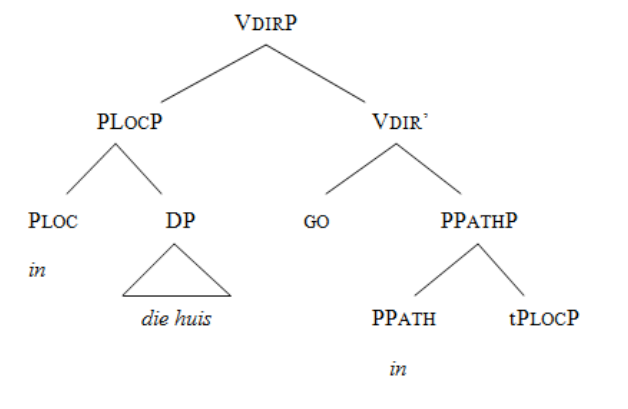
\includegraphics[width=\textwidth]{figures/biberauer43.png}
\begin{forest}
[V\textsubscript{\textsc{dir}}P [P\textsubscript{\textsc{loc}}P [P\textsubscript{\textsc{loc}}\\\textit{in},align=center] [DP [\textit{die huis},roof] ] ]  [V\textsubscript{\textsc{dir}'} [\textsc{go}] [P\textsc{path}P [P\textsc{path}\\\textit{in},align=center] [\textit{t}P\textsc{\textsubscript{loc}}P]] ] ] 
\end{forest}

\z
 


In \REF{ex:biberauer:42}, we see directionally interpreted structures that superficially lack a lexical verb.  \Citet{vanRiemsdijk2002} provides convincing argumentation that this is only apparently the case, and that a silent motion verb, \textsc{go,} is in fact present in the structure. If this silent verb is also present in \isi{directional} circumpositional structures like \REF{ex:biberauer:41} and in \isi{directional} postpositional structures more generally, we can understand why the “postpositions” in both types of \isi{directional} structures are not in fact postpositions at all. Consider \REF{ex:biberauer:43} to see why this is so. In this simplified structure, we follow \citet{denDikken2010pps,denDikken2010getgo} in assuming a PP-structure in which P\textsc{\textsubscript{Loc}}P is selected by P\textsc{\textsubscript{Path}}P which is, in turn, potentially dominated by P\textsc{\textsubscript{Dir}}P (see also \citealt{Koopman2010} for a variant of this proposal). The presence of silent \textsc{go}, however, raises the possibility of structures in which the \isi{directionality} component is represented not by a fully-fledged P\textsc{\textsubscript{Dir}}P, but instead, by a V that incorporates \textsc{\textsubscript{Dir}}, the silent V\textsc{\textsubscript{Dir}}\textsc{ go,} i.e. a structure in which the PP-component is defective, with part of what PPs can contribute to \isi{directional} meaning being contributed by the verbal entity with which they combine rather than by the PP itself.\footnote{\label{fn:biberauer:39}%
In \citet{Pretorius2015}, these options are conceived of as the consequence of different ‘spanning’ choices (cf. \citealt{Svenonius2011,Svenonius2016}).} Significantly in the current context, this structure does not violate \REF{ex:biberauer:6}-type FOFC\is{Final-over-Final Condition}.

That \isi{directional} postpositions appear to be defective compared to locative prepositions has already been demonstrated in (\ref{ex:biberauer:35}--\ref{ex:biberauer:36}) above, and the same discrepancy emerges when we consider the few \isi{directional} prepositions in \ili{Afrikaans} relative to their postpositional counterparts. Contrast \REF{ex:biberauer:44} with \REF{ex:biberauer:36}, repeated here as \REF{ex:biberauer:45}, for example:

\ea%44
    \label{ex:biberauer:44}
    \ea 
\gll Hy het \textbf{na} \textbf{die} \textbf{swembad}          gehardloop.\\
    he  has to  the swimming.pool run\\
  \glt ‘He ran to the swimming pool.’

 \ex
\gll Hy het gehardloop \textbf{na} \textbf{die} \textbf{swembad}.{\rmfnm}\\
    he  has run             to   the swimming.pool\\
\z
\z
\footnotetext{\label{fn:biberauer:40}Significantly, the circumpositional variant of this structure, in which \textit{na} is reinforced by \textit{toe} – \textit{Hulle het gehardloop na die swembad toe} – is also readily acceptable, in sharp contrast to the pattern to be discussed below and illustrated in \REF{ex:biberauer:44}. We return to this matter below.}

\ea%45
    \label{ex:biberauer:45}
    \ea
    \gll   Hulle het     die bos    \textbf{in}    geloop.{}    \\
	    they  have   the bush  in    walked\\
    \glt  ‘They walked into the bush.’
  
 \ex 
\gll  *Hulle het    geloop  die bos   \textbf{in}.\\
      they   have walked the  bush in\\
\z
\z

While prepositional \textit{na}{}-PPs can extrapose, postpositional \textit{in}{}-phrases like those in (\ref{ex:biberauer:36}\slash \ref{ex:biberauer:45}b) cannot.   \citet{AelbrechtdenDikken2013} propose that the P\textsc{\textsubscript{Dir}}P-component of identical doubling structures lacks the full functional structure associated with the locative component of the circumposition: in lexicalization (and also “spanning”; see note \ref{fn:biberauer:39}) terms, we can think of this as doubling Ps being unspecified for \textsc{dir}, with the result that they cannot themselves project P\textsc{dir}P (\textit{in} in (\ref{ex:biberauer:43}) is the head of P\textsc{PathP}). Here, we propose that this is also more generally true of \isi{directional} postpositions in \ili{Afrikaans} (and in \ili{West Germanic} more generally). 

This has two immediate consequences. The first of these is that P\textsc{\textsubscript{Path}} will incorporate with V\textsc{\textsubscript{dir}}\textsc{,} and, from there, into the lexical verb with which the V\textsc{\textsubscript{dir}}{}-structure is ultimately merged. Assuming the approach to incorporation in \citet{Roberts2010agreement}, P\textsc{\textsubscript{Path}} constitutes a defective goal in relation to V\textsc{\textsubscript{dir}}, as it lacks the \textsc{dir}{}-specification present on the latter head;\footnote{If P\textsubscript{PATH} is to constitute a defective goal in Roberts’ terms, it has to be assumed that its categorial status will not render it partially distinct from V\textsc{\textsubscript{dir}}\textsc{.} Precisely how the formal specification of “what it means to be a V” versus “what it means to be a P” is to be captured is not a matter on which there is currently any consensus. What is clear, however, is the empirical fact that certain P-elements, like certain predicative nominal elements, can incorporate into verbal elements; if \citet{Roberts2010agreement} is correct in analyzing incorporation as involving the presence of defective goals, we can use cases like those under discussion here to make progress on long-standing questions about the categorial make-up of P-elements.} the incorporated P\textsc{\textsubscript{Path}}{}-V\textsc{\textsubscript{dir}}{}-structure, in turn, is plausibly a defective goal in relation to the lexical verb, which will bear verbal specifications typical of fully-fledged overt lexical items (cf. again the references cited above on the idea that null elements lack properties associated with their overt “counterparts”, and i.a. \citealt{Pesetsky1995} and  \citealt{BoškovićLasnik2003}). Taken together, these incorporations predict that postpositional Ps in \ili{Afrikaans} (and \ili{Dutch}) will always precede the lexical verb. This, in turn, allows us to understand why extraposition structures such as those in (\ref{ex:biberauer:36}/\ref{ex:biberauer:45}b) are barred: postpositional \textit{in} must incorporate with a higher verbal head in order to be licensed, and, as such, cannot surface in the kind of non-adjacent, rightward position that extraposition structures would require. Further, thanks to this dependence on the relevant lexical verbs, the P-V combinations are recognized by native-speakers as (separable) particle verbs of the transparent (rather than idiomatic; cf. \citealt{Wurmbrand2000}) kind. 

The second immediate consequence is that we can understand the unavailability of \ili{Afrikaans} (and \ili{Dutch}) postpositional PP-extraposition as another manifestation of a more widely observed pattern in terms of which only “full” structures are extraposable (cf. i.a. \citealt[294]{Wurmbrand2001}, \citealt[15]{Hinterhölzl2005},  \citealt[32ff]{BiberauerSheehan2012}, and  \citealt[8--9]{SheehanVanderWal2015} for different versions of this idea). In \ili{West Germanic} and many other OV-systems, for example, we observe that full CP-complements surface in postverbal position (cf. again \REF{ex:biberauer:4} above, and \REF{ex:biberauer:46a} below), while reduced clausal complements necessarily appear to the left of the verb \REF{ex:biberauer:46b}:

\ea%46
\label{ex:biberauer:46} 
\ea []{\label{ex:biberauer:46a}  (\ili{German})\\
\gll Es scheint, [\textsc{\textsubscript{CP}} \textbf{dass} der Hans sich rasiert].      \\
    it   seems    ~     that  the John  self shaves\\
  \glt ‘It seems that John is shaving himself.’}

 \ex[]{\label{ex:biberauer:46b} 
\gll   ... dass Hans [\textsubscript{TP} sich zu rasieren] schien. \\
      ~  that  Hans   ~   self  to shave      seemed \\
\glt ‘… that Hans seemed to shave himself.’}

 \ex[*]{
\gll   … dass Hans schien [\textsubscript{TP} sich zu rasieren]. \\
        ~  that  Hans seemed  ~   self to  shave\\}
\z
\z

If, as we have argued above, postpositional (\isi{directional}) Ps lack the full functional structure associated with prepositional Ps, – which are mostly, but not exclusively locative; cf. \textit{na} in \REF{ex:biberauer:44} – we expect prepositional PPs to be extraposable, while postpositional PPs are not. Further, we also expect the pattern in \REF{ex:biberauer:47}, which would be puzzling if extraposition simply rested on the presence versus absence of a preposition-containing PP:

\ea%47
    \label{ex:biberauer:47}
     \ea[]{\label{ex:biberauer:47a}
\gll  Hulle het   \textbf{by/in} \textbf{die} \textbf{bos} \textbf{in} geloop.\\
    They have by/in  the bush in walked\\
  \glt ‘They walked into the bush.’}

 \ex[*]{\label{ex:biberauer:47b}
\gll  Hulle het    geloop \textbf{by/in} \textbf{die} \textbf{bos} \textbf{in}.\\
      they   have walked by/in the  bush in\\}

 \ex[]{\label{ex:biberauer:47c}
\gll   Hulle het    \textbf{in}geloop  \textbf{by/in} \textbf{die} \textbf{bos}.{\rmfnm}\\
    they   have in.walked by/in  the bush\\
  \glt ‘They walked into the bush.’}
\z
\z
\footnotetext{Importantly, \textit{Hulle het ingeloop in die bos} in \REF{ex:biberauer:47c} means ‘They walked into the bush’, like \REF{ex:biberauer:47a}, and not ‘They walked in the bush’, like \REF{ex:biberauer:35b}, \textit{Hulle het geloop in die bos}.}

Here we see that circumpositional \isi{directional} PPs mirror the behaviour of their postpositional counterparts (\ref{ex:biberauer:36}/\ref{ex:biberauer:45}b) in resisting extraposition \REF{ex:biberauer:47b}, despite the presence of a \isi{preposition}. Significantly, extraposition of the (locative) prepositional component of the structure becomes possible where the \isi{postposition} is immediately left-adjacent to the verb \REF{ex:biberauer:47c}, i.e. where, in our terms, it has incorporated, via V\textsc{\textsubscript{dir}} (cf. \ref{ex:biberauer:43} above), with the lexical verb and thus been licensed by it.\footnote{Interestingly, this structure may at first sight seem to resemble the extraposition pattern predicted by \citegen{Sheehan2013fofc} FOFC\is{Final-over-Final Condition} analysis (see again \sectref{sec:biberauer:2} above). As it is very clearly the \textit{post}position that precedes the verb, with the prepositional PP following it, this is not a possible analysis of the structure, however. This is demonstrated in (i), which shows the scattered-deletion operation that would be expected on this approach:

\ea
\gll Hulle het    \textbf{by/in} \sout{\textbf{die} \textbf{bos} \textbf{in}} geloop \sout{\textbf{by/in}} \textbf{die} \textbf{bos} \textbf{in}.\\
they   have by/in  the bush in walked by/in the  bush in\\
\z
}  In this case, the prepositional PP, which is, as always, a complete phasal structure, may extrapose; in \REF{ex:biberauer:47b}, by contrast, extraposition is barred because postpositional \textit{in}, located on top of the fully phasal prepositional PP, is defective, meaning the circumpositional structure as a whole is non-phasal and thus, by hypothesis, non-extraposable. An appealing way to think about what is at stake here is via \citegen{SheehanVanderWal2015} Extend licensing mechanism, given in \REF{ex:biberauer:48}:

\ea%48
    \label{ex:biberauer:48}
	  Extend: All categories must be part of a \isi{phase} (where phases include vP, CP\is{complementizer}, nP, DP, pP, and its CP-/upper-\isi{phase} counterpart – MTB).
\z

In terms of this plausibly interface-imposed requirement, incorporation into V in cases like \REF{ex:biberauer:47c} allows defective \isi{directional} \textit{in}, which lacks its own functional structure, to satisfy \REF{ex:biberauer:48}: via incorporation, it becomes part of the vP-\isi{phase}. Because postpositional \textit{in} is not part of a (complete) \isi{phase} prior to incorporation with V, it is not extraposable along with the lower (prepositional) \isi{phase} of the PP-structure it is first-merged with. 


As registered in note \ref{fn:biberauer:40}, \textit{na … toe} circumpositions constitute an exception to the pattern illustrated in \REF{ex:biberauer:47}: a \textit{na … toe} circumposition can extrapose, unlike \textit{by/in die bos in} in \REF{ex:biberauer:47b}. Strikingly, we also do not see incorporation of the type in \REF{ex:biberauer:47c} with \textit{na … toe} circumpositions. This is shown in \REF{ex:biberauer:49}, which is interpretively equivalent to \REF{ex:biberauer:44} above:



\ea%49
    \label{ex:biberauer:49}
	  \ea  \label{ex:biberauer:49a}
\gll Hulle het    \textbf{na} \textbf{die} \textbf{swembad} \textbf{toe}  gehardloop.\\
    they   have to  the swimming.pool to    run\\
  \glt ‘They ran to the swimming pool.’
 \ex \label{ex:biberauer:49b}
\gll   Hulle het   gehardloop \textbf{na} \textbf{die} \textbf{swembad} \textbf{toe}.\\
    they   have run             to  the  swimming.pool to\\
  \glt ‘They ran to the swimming pool.’
 \ex \label{ex:biberauer:49c}
\gll   *Hulle het    \textbf{toe}gehardloop na die swembad.\\
      they   have to.run               to  the swimming.pool\\
\z
\z



An immediate difference between \REF{ex:biberauer:47a} and \REF{ex:biberauer:49a} is that the \isi{preposition} in \REF{ex:biberauer:49}, \textit{na}, is already inherently \isi{directional}, i.e. \textsc{dir}{}-bearing; postpositional \textit{toe} thus simply echoes its \isi{directional} meaning in a manner semantically, though not lexically, reminiscent of the so-called \ili{German} \textit{shadow Ps} discussed in \citet{Noonan2010}. Further \textit{toe} is one of the alternating P-forms in \ili{Afrikaans}: like \textit{vir/voor} illustrated in (\ref{ex:biberauer:37}--\ref{ex:biberauer:38}) above, it consistently takes a different form (\textit{toe}) when it surfaces postnominally to that which we see when it occurs prenominally (\textit{tot});\textit{ met/mee} (‘with’) is the final member of this trio. \REF{ex:biberauer:50} illustrates the alternation between \textit{tot} and \textit{toe}.



\ea%50
    \label{ex:biberauer:50}
     \ea\label{ex:biberauer:50a}
\gll  Sy  het \textbf{tot} [\textsubscript{PP} by die see] gehardloop (en    daarna       omgedraai).\\
    she has to   ~    by the sea   run               {\db}and  there.after around.turned\\
  \glt ‘She ran to the sea and then turned around.’
 \ex\label{ex:biberauer:50b}
\gll  Sy  het  see \textbf{toe} gehardloop.\\
    she has sea to    run \\
  \glt ‘She ran to(wards) the sea.’
\z
\z


As noted above,   \citet{DeVos2013} analyses this alternation as signifying a difference between agreeing\is{agreement} (\textit{voor/toe/mee}) and non-agreeing\is{agreement} (\textit{vir/tot/met}) prepositions. Building, on the one hand, on this insight and on the idea that \isi{agreement} is a property of a non-defective phasal domain (cf. i.a. \citealt{Chomsky2001}), and, on the other, on the observation that \textit{toe} differs from \textit{tot} in giving non-telic \isi{directional} interpretations, we propose that \textit{toe} differs from the (particle) postpositions discussed to date in (i) being part of a non-defective upper (i.e. \isi{directional}) phasal domain, and (ii) selecting a defective \textit{lower} (i.e. locative) phasal domain. More specifically, I propose that \textit{toe} is a P\textsc{\textsubscript{path}}{}-head which consistently selects a nominal headed by silent \textsc{place} (cf. \citealt{Kayne2008expletives}); see \REF{ex:biberauer:52b} below. This nominal and the overt nominal structure it introduces are then always available for probing (and, in keeping with phi-probing heads in \ili{Afrikaans} more generally,\footnote{\label{fn:biberauer:44}%
v, T and C can all be viewed as phi-probes which raise the nominals they probe. Prepositional Ps would then be an exception to this generalization. Since agreeing\is{agreement} Ps are crosslinguistically unusual, it is tempting to think that selection relations between Ps and their complements do not typically involve phi, with the cases where we do see \isi{agreement} signifying a departure from this norm. This would, of course, require rethinking of P’s role as a licensor, with \citegen{SheehanVanderWal2015} approach presenting a possible way forward.}  subsequent movement) by the agreement-bearing P\textsc{\textsubscript{Path}}{}-head that is ultimately spelled out as \textit{toe}. A simplified version of the proposed derivation is schematized in \REF{ex:biberauer:51} (strikethrough signifies a non-spelled-out lower copy, as before; the probing P\textsc{\textsubscript{Dir}}{}-phasehead remains unrealized in \REF{ex:biberauer:50b}, but see \REF{ex:biberauer:52} below for the overt realization option, which represents an innovation in \ili{Afrikaans}):



\ea%51
    \label{ex:biberauer:51}
	  [\textsubscript{P\textsc{dir}P} \textsc{dir}… 
	    [\textsubscript{P\textsc{path}P}  
	      [\textsubscript{DP} \textsc{place} 
		[\textsubscript{NP} \textit{see}] 
	      ] \textsc{Path-}\textit{toe} 
	      [\textsubscript{DP} \textsc{place} 
		[\textsubscript{NP} \textit{see}] 
	      ]
	    ]
	  ]
\z


\textit{Tot}, by contrast, selects a non-defective locative complement, necessarily introduced by an overt \isi{preposition} (e.g. \textit{by} in (\ref{ex:biberauer:50a})\footnote{Temporal \textit{tot} – e.g. \textit{tot Maandag}, ‘until Monday’ – is different, systematically selecting nominals.}), and lacks the phi-probe associated with \textit{toe}, a factor which does not, however, render it defective in phasal terms, as the extraposition facts clearly show (see note \ref{fn:biberauer:44} on the relation between P and phi); \textit{tot} instead appears to lexicalize both \textsc{Path} and \textsc{Dir}, suggesting that it may be the spellout of a composite head, i.e. both \textsc{Path} and \textsc{Dir} in \REF{ex:biberauer:51} above.



Significantly, the analysis proposed here means that \textit{toe} in structures like \REF{ex:biberauer:49} does not in fact combine with a PP headed by \textit{na}, i.e. \textit{na … toe} structures do not involve a FOFC-violating final-over-initial configuration and are actually very different from the superficially very similar identical doubling circumpositions discussed above. The difference is schematized in \REF{ex:biberauer:52}:


\ea%52
    \label{ex:biberauer:52} 
\ea (=\ref{ex:biberauer:43})  \label{ex:biberauer:52a}
\begin{forest}
[V\textsubscript{\textsc{dir}}P [P\textsubscript{\textsc{loc}}P [P\textsubscript{\textsc{loc}} [\textit{in},no edge,tier=word]] [DP [\textit{die huis},roof,tier=word] ] ]  [V\textsubscript{\textsc{dir}'} [\textsc{go}] [P\textsc{path}P [P\textsc{path} [\textit{in}, no edge, tier=word]] [tPlocP]] ] ] 
\end{forest}
% 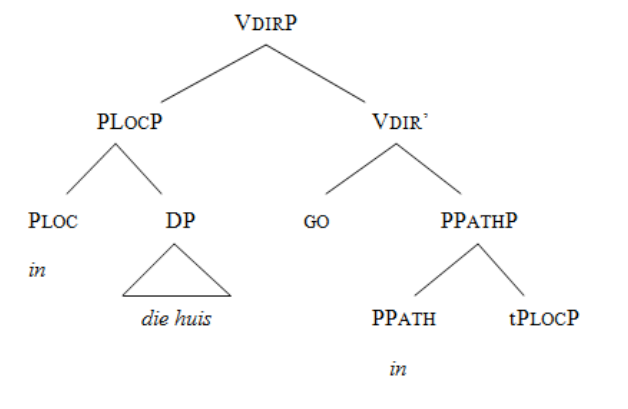
\includegraphics[width=\textwidth]{figures/biberauer52a.png} 
\ex \label{ex:biberauer:52b}
\begin{forest}
[P\textsubscript{\textsc{dir}}P [P\textsubscript{\textsc{dir}}\\\textit{na},base=top,align=center] [P\textsubscript{\textsc{path}}P [\textsc{PlaceP} [\textsc{Place}] [\textsc{dp} [\textit{die see},roof,tier=word] ] ] [\isi{Path}' [\isi{Path} [\textit{toe},no edge, tier=word] ] [t\textsc{PlaceP}] ] ] ]
\end{forest}
% 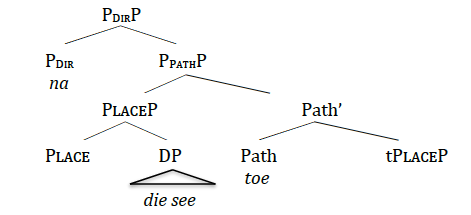
\includegraphics[width=\textwidth]{figures/biberauer52b.png}
\z
\z



The proposal for \ili{Afrikaans} circumpositions, then, is that they come in two types. The first and most common type is that illustrated in \REF{ex:biberauer:52a}, in which the superficial \isi{postposition} is not in fact part of a PP-structure, but is instead part of a particle-verb structure in which the \isi{directional} component is contributed by silent V\textsc{\textsubscript{dir}}\textsc{ go.} Not expressing \textsc{dir} itself, this defective P-element incorporates into V\textsc{\textsubscript{dir}} and, from there, into the lexical verb, which allows it to become part of a non-defective phasal domain (vP); the fact that it necessarily surfaces adjacent to the lexical verb and cannot be extraposed as part of a circumpositional structure thus follows. This type is also found in \ili{Dutch}, mostly in the non-doubling form  (e.g. \textit{by die bos in} as in (\ref{ex:biberauer:47})), but also in some varieties in the doubling form found in \ili{Afrikaans} (i.e. the \textit{in die bos in}{}-variant of \REF{ex:biberauer:47}; cf. the Asse \ili{Dutch} example in (\ref{ex:biberauer:41b})). The second type is an innovation in \ili{Afrikaans} and involves a genuine circumpositional structure. This is, however, not a FOFC-violating structure either as head-initial \textit{na} dominates head-final \textit{toe}, as shown in \REF{ex:biberauer:52b}. The Ps in this structure are both non-defective, with the result that we expect it to be able to extrapose as in \REF{ex:biberauer:49b}; since the postpositional element is structurally too distant from the lexical verb to undergo incorporation, the ungrammaticality of \REF{ex:biberauer:49c} above is also expected. \ili{Afrikaans}, then, does not present any challenges to \REF{ex:biberauer:6}-type FOFC\is{Final-over-Final Condition}. 


\subsection{A brief look at circumpositions beyond Afrikaans}


We do not have the space to demonstrate this here, but it appears to be the case that \ili{Afrikaans}’ \ili{West Germanic} relatives do not present additional FOFC\is{Final-over-Final Condition} challenges: the majority appear to feature only particle-type postpositions and, thus, lack genuine final-over-initial PP-structures as the structure in {question} is that illustrated in (\ref{ex:biberauer:43}\slash \ref{ex:biberauer:52a}). Worth noting, though, is the fact that the varieties of colloquial \ili{German} that permit the shadow Ps analysed in \citet{Noonan2010} and illustrated in \REF{ex:biberauer:53} appear to mirror \ili{Afrikaans} in featuring both \REF{ex:biberauer:52a}- and \REF{ex:biberauer:52b}-type circumpositional structures, with the shadow-containing circumpositions instantiating the latter type:



\ea%53
    \label{ex:biberauer:53}
    

	 \ea
\gll  \textbf{in} der Kiste \textbf{drin} \\
in the box    DR-in\\
\glt ‘inside the box’      (=locative; \citealt[164]{Noonan2010})



 \ex
\gll   \textbf{um}     den Tisch  \textbf{rum}\\
   round the   table  R-round\\
  \glt ‘around the table’      (=\isi{directional}; \citealt[169]{Noonan2010})
\z
\z


The \ili{Gbe} languages discussed in \citet{Aboh2005,Aboh2010}, in turn, appear only to feature the \REF{ex:biberauer:52b}-type, i.e. initial-over-final, inverse FOFC\is{Final-over-Final Condition} structures. In fact, this language family facilitates particularly clear insight into how different the P-elements in circumpositional structures can be. Consider \REF{ex:biberauer:54}:



\ea%54
    \label{ex:biberauer:54}
  	 \ea
\gll  Kɔjó zé    àkwɛ   \textbf{xlán} Kwésí.          [\ili{Gungbe}]\\
    Kojo take money P\textsubscript{1}   Kwesi\\
  \glt ‘Kojo sent money to Kwesi.’



 \ex
\gll  Kɔjó  xɛ      távò  lɔ    \textbf{jí}.\\
    Kojo climb table \textsc{det} P\textsubscript{2}\\
\glt ‘Kojo climbed on top of the table.’

\ex
\gll  Kpònɔn lɛ     nyì     àgbàn    cè     \textbf{xlán} gbó    \textbf{jí}.\\
 police   \textsc{num} throw luggage \textsc{poss} P\textsubscript{1}     trash P\textsubscript{2}\\
\glt ‘The policemen threw my luggage onto the dumpster.’
\citep[227]{Aboh2010}
\z
\z





As Aboh demonstrates, the prepositional Ps (P\textsubscript{1}) behave consistently differently from the postpositional Ps (P\textsubscript{2}). The former evidently constitute a small closed class of 5 members all expressing direction/goal/path, all derive from verbs (possibly via serial constructions), seem to assign \isi{Case}, and, rather unusually given the crosslinguistic trend, must necessarily be stranded. The latter, in turn, are all derived from nouns and closely resemble the elements \citet{Jackendoff1996} originally designated \textit{Axial Parts};\footnote{\citet[14]{Jackendoff1996} clarifies the notion ``Axial Part'' as follows: ‘The “axial parts” of an object – its top, bottom, front, back, sides, and ends – behave grammatically like parts of the object, but, unlike standard parts such as a handle or a leg, they have no distinctive shape. Rather, they are \textit{regions} of the object (or its boundary) \textit{determined by} their \textit{relation to the object’s axes}. The up-down axis determines top and bottom, the front-back axis determines front and back, and a complex set of criteria distinguishing horizontal axes determines sides and ends.’ (my emphasis –TB)} there are about 30 of them, they do not assign \isi{Case}, and they must be piedpiped. Following \citegen{Svenonius2006axialparts} characterization of Ax(ial)PartP as a nominal-peripheral (‘light noun’) \isi{projection} located below the P-layers expressing location and direction \REF{ex:biberauer:55a}, \ili{Gungbe} circumpositions will be initial-over-final structures \REF{ex:biberauer:55b}, with the finality of the high nominal layer being unproblematic in view of \ili{Gungbe}’s head-final nominal system \REF{ex:biberauer:55c}:

\ea \label{ex:biberauer:55}
\ea \label{ex:biberauer:55a}
  \textit{pP} > LocP > \textbf{AxPartP} > KP > DP    
 \ex \label{ex:biberauer:55b}
  \textit{P}\textit{\textsubscript{1}}\textit{P (direction/goal/path)} > \textbf{P}\textbf{\textsubscript{2}}\textbf{P} \citep{Aboh2010}

 \ex \label{ex:biberauer:55c}
\gll   Mì   fɔn     hàɖòkpólɔ     \textit{sɔn} \textbf{zàn} \textbf{lɔ}      jí!\\
  \textsc{2pl}  stand  immediately P\textsubscript{1}   bed  \textsc{Det}  P\textsubscript{2}\\

\glt ‘Get out of the bed immediately!’     \citep[229]{Aboh2010}
\z 
\z

Neither the \ili{West Germanic} nor the \ili{Gbe} languages, then, appear to constitute a challenge to FOFC\is{Final-over-Final Condition} as defined in \REF{ex:biberauer:6}. Interestingly, they do not challenge Richards’s more restrictive phasal-domain-based definition either (see \sectref{sec:biberauer:2}) as we have seen that none of the superficially problematic structures we have considered here involves a final head dominating an initial one that is located in the same spellout domain. What is striking about the adpositional facts discussed here, however, is the way in which Extended\is{extended projection} Projections repeatedly emerge as a relevant consideration in characterizing the structure of the observed phenomena: in some cases, postpositions can be shown to be defective, lacking the higher functional structure that would lead to their forming part of a complete phasal domain, with the result that they incorporate into another lexical category (here: V) and become part of a second Extended \isi{Projection}\is{extended projection} (possibly, in line with Extend, as given in \REF{ex:biberauer:48}; this holds for particle-type postpositions as in \ref{ex:biberauer:43}\slash\ref{ex:biberauer:52}a); in others, functional structure \textit{below} the final element is defective, meaning that we again have a defective Extended \isi{Projection}\is{extended projection} (this holds for \REF{ex:biberauer:52b}-type postpositions). That apparently FOFC-violating structures should repeatedly exhibit some kind of Extended\is{extended projection} Projection-related peculiarity is precisely what is expected on the restricted condition in \REF{ex:biberauer:6}, while it is unexplained on Richards’ phasal-domain alternative.\footnote{It is worth noting that acknowledging the significance of defectivity in the FOFC context also seems like an important step in facilitating progress on the intriguing {question} of why VOC should be completely barred where C is a subordinating Complementizer\is{complementizer} of the kind considered in typological studies since \citeauthor{greenberg1963} (1963; see again \citealt{Dryer2009} for overview discussion) while it seems extremely common where C is some kind of particle; and, similarly, why inflecting auxiliaries obey FOFC\is{Final-over-Final Condition}, while their particle counterparts do not. If the conforming elements contribute to Extended\is{extended projection} Projections, while particle elements do not, the discrepancy becomes less mysterious (see \citealt{Biberauer2017optionalv2} for discussion).} The internal structure of apparently FOFC-violating PPs, we contend, therefore provides another argument in favour of this intermediate interpretation of FOFC\is{Final-over-Final Condition}’s restrictiveness. 

\section{Conclusion}\label{sec:biberauer:5}

Our objective in this paper was to take a closer look at adpositional phrases in order to establish what kinds of insights these may add to our understanding of a by now much-discussed word-order condition, FOFC\is{Final-over-Final Condition}. Adpositions present numerous superficial challenges to FOFC\is{Final-over-Final Condition}, in both of its most familiar formulations, \REF{ex:biberauer:1} and \REF{ex:biberauer:6} above. Closer inspection of, on the one hand, the external distribution of PPs in OV-languages and, on the other, the internal make-up of post- and circumpositional PPs suggests that the latter, which crucially makes reference to Extended\is{extended projection} Projections, seems the most promising. The data we have considered reveals a range of ways in which postpositions and circumpositional structures can be unproblematic in the FOFC\is{Final-over-Final Condition} context. This is the same finding as that which has emerged from closer investigation of two other domains in which apparently FOFC-violating structures seem to abound, final particle-containing structures \citep{Biberauer2017optionalv2}, and 231 verb-clusters in \ili{West Germanic} \citep{Biberauer2013}. In each case, it has proven productive to investigate each apparently problematic structure independently as it has become clear that apparently FOFC-violating structures can arise from quite diverse underlying structures (hence also their (relatively) frequent attestation); and, in each case, it has emerged either that there are reasons to reject the possibility that the troublesome final elements examined form part of the same Extended \isi{Projection}\is{extended projection} as lower head-initial elements, or that the underlying structure is in fact the inverse-FOFC\is{Final-over-Final Condition} (initial-over-final) one. Many cases still require detailed investigation, but, at this stage, the hypothesis that something like the restricted, crucially Extended\is{extended projection} Projection-based FOFC\is{Final-over-Final Condition} defined in \REF{ex:biberauer:6} may indeed be \isi{universal} remains promising. 

If this is correct, FOFC\is{Final-over-Final Condition} is a ‘deep’ \isi{universal}, constituting a condition on syntactic structure-building that has wide-ranging consequences for word order. This makes it, in the terms of \citet{Whitman2008}, both a cross-categorial generalization – i.e. ‘one that references the internal properties of two or more categories, irrespective of their relationship in a particular structure’ (233); Greenberg’s Universal 3 is an example\footnote{\textbf{Universal 3:} Languages with dominant VSO order are always prepositional \citep[78]{greenberg1963}.} – and a hierarchical generalization – i.e. ‘one that describes the relative position of two or more categories in a single structure’ (234); Greenberg’s Universal 1 is an example.\footnote{\textbf{Universal 1:} In declarative sentences with nominal subject and object, the dominant order is always one in which the subject precedes the object.} For Whitman, cross-categorial and hierarchical generalizations are very different, with only the latter being ‘deep’ (in hierarchical terms, Universal 3 follows from the \isi{universal} leftness of specifiers; cf. i.a. \citealt{Kayne1994}, \citealt{AckemaNeeleman2002}, and \citealt{BiberauerEtAl2014nochoice}). 
FOFC\is{Final-over-Final Condition}, however, would seem to be a hybrid of two of the generalization-types identified by Whitman, a truly novel kind of 
syntactic \isi{universal}, the existence of which was first registered by the linguist to whom this volume is dedicated, Anders Holmberg.
 

\section*{Abbreviations}
Abbreviations used in this article follow the Leipzig Glossing Rules’ instructions for word-by-word transcription, available at: \url{https://www.eva.mpg.de/lingua/pdf/Glossing-Rules.pdf}.

\section*{Acknowledgements}
This paper is based on a presentation at the International Workshop on Adpositions, organized by Anders Holmberg and Sameerah Saheed and held at the University of Newcastle in June 2014. Thanks to the audience for their comments and suggestions, to Erin Pretorius for subsequent (and on-going) discussions of matters {Afrikaans} PP-related, and to Ian Roberts and two anonymous reviewers for input that has hopefully led to a sharpening of some of the ideas in this paper. 


{\sloppy\printbibliography[heading=subbibliography,notkeyword=this]}
\end{document}